
% I seguenti commenti speciali impostano:
% 1. 
% 2. PDFLaTeX come motore di composizione;
% 3. tesi.tex come documento principale;
% 4. il controllo ortografico italiano per l'editor.

% !TEX encoding = UTF-8
% !TEX TS-program = pdflatex
% !TEX root = tesi.tex
% !TEX spellcheck = it-IT

\documentclass[10pt,                    % corpo del font principale
               a4paper,                 % carta A4
               twoside,                 % impagina per fronte-retro
               openright,               % inizio capitoli a destra
               english,                 
               italian,                 
               ]{book}    

\usepackage[utf8]{inputenc}             % codifica di input; anche [latin1] va bene
                                        % NOTA BENE! va accordata con le preferenze dell'editor

%**************************************************************
% Importazione package
%************************************************************** 

%\usepackage{amsmath,amssymb,amsthm}    % matematica

\usepackage[english, italian]{babel}    % per scrivere in italiano e in inglese;
                                        % l'ultima lingua (l'italiano) risulta predefinita

\usepackage{bookmark}                   % segnalibri

\usepackage{caption}                    % didascalie

\usepackage{chngpage,calc}              % centra il frontespizio

\usepackage{csquotes}                   % gestisce automaticamente i caratteri (")

\usepackage{emptypage}                  % pagine vuote senza testatina e piede di pagina

\usepackage{epigraph}					% per epigrafi

\usepackage{eurosym}                    % simbolo dell'euro

\usepackage[T1]{fontenc}                % codifica dei font:
                                        % NOTA BENE! richiede una distribuzione *completa* di LaTeX

%\usepackage{indentfirst}               % rientra il primo paragrafo di ogni sezione

\usepackage{graphicx}                   % immagini

\usepackage{hyperref}                   % collegamenti ipertestuali



\usepackage[binding=5mm]{layaureo}      % margini ottimizzati per l'A4; rilegatura di 5 mm

\usepackage{listings}                   % codici

\usepackage{microtype}                  % microtipografia

\usepackage{mparhack,fixltx2e,relsize}  % finezze tipografiche

\usepackage{nameref}                    % visualizza nome dei riferimenti                                      

\usepackage[font=small]{quoting}        % citazioni

\usepackage{subfig}                     % sottofigure, sottotabelle

\usepackage[italian]{varioref}          % riferimenti completi della pagina

\usepackage[dvipsnames]{xcolor}         % colori

\usepackage{booktabs}                   % tabelle                                       
\usepackage{tabularx}                   % tabelle di larghezza prefissata                                    
\usepackage{longtable}                  % tabelle su più pagine                                        
\usepackage{ltxtable}                   % tabelle su più pagine e adattabili in larghezza

\usepackage[toc, acronym]{glossaries}   % glossario
                                        % per includerlo nel documento bisogna:
                                        % 1. compilare una prima volta tesi.tex;
                                        % 2. eseguire: makeindex -s tesi.ist -t tesi.glg -o tesi.gls tesi.glo
                                        % 3. eseguire: makeindex -s tesi.ist -t tesi.alg -o tesi.acr tesi.acn
                                        % 4. compilare due volte tesi.tex.

\usepackage[backend=bibtex,style=verbose-ibid,hyperref,backref]{biblatex}
                                        % eccellente pacchetto per la bibliografia; 
                                        % produce uno stile di citazione autore-anno; 
                                        % lo stile "numeric-comp" produce riferimenti numerici
                                        % per includerlo nel documento bisogna:
                                        % 1. compilare una prima volta tesi.tex;
                                        % 2. eseguire: biber tesi
                                        % 3. compilare ancora tesi.tex.

%**************************************************************
% file contenente le impostazioni della tesi
%**************************************************************

%**************************************************************
% Frontespizio
%**************************************************************

% Autore
\newcommand{\myName}{Pier Paolo Tricomi (Matr. 1096827)}                                    
\newcommand{\myTitle}{Sviluppo di un sistema per la gestione e il controllo di licenze software}

% Tipo di tesi                   
\newcommand{\myDegree}{Tesi di laurea triennale}

% Università             
\newcommand{\myUni}{Università degli Studi di Padova}

% Facoltà       
\newcommand{\myFaculty}{Corso di Laurea in Informatica}

% Dipartimento
\newcommand{\myDepartment}{Dipartimento di Matematica "Tullio Levi-Civita"}

% Titolo del relatore
\newcommand{\profTitle}{Prof. }

% Relatore
\newcommand{\myProf}{Mauro Conti}

% Luogo
\newcommand{\myLocation}{Padova}

% Anno accademico
\newcommand{\myAA}{2016-2017}

% Data discussione
\newcommand{\myTime}{Settembre 2017}


%**************************************************************
% Impostazioni di impaginazione
% see: http://wwwcdf.pd.infn.it/AppuntiLinux/a2547.htm
%**************************************************************

\setlength{\parindent}{14pt}   % larghezza rientro della prima riga
\setlength{\parskip}{0pt}   % distanza tra i paragrafi


%**************************************************************
% Impostazioni di biblatex
%**************************************************************
\bibliography{bibliografia} % database di biblatex 

\defbibheading{bibliography} {
    \cleardoublepage
    \phantomsection 
    \addcontentsline{toc}{chapter}{\bibname}
    \chapter*{\bibname\markboth{\bibname}{\bibname}}
}

\setlength\bibitemsep{1.5\itemsep} % spazio tra entry

\DeclareBibliographyCategory{opere}
\DeclareBibliographyCategory{web}

\addtocategory{opere}{womak:lean-thinking}
\addtocategory{web}{site:agile-manifesto}

\defbibheading{opere}{\section*{Riferimenti bibliografici}}
\defbibheading{web}{\section*{Siti Web consultati}}


%**************************************************************
% Impostazioni di caption
%**************************************************************
\captionsetup{
    tableposition=top,
    figureposition=bottom,
    font=small,
    format=hang,
    labelfont=bf
}

%**************************************************************
% Impostazioni di glossaries
%**************************************************************

\label{cap:glossario}
%**************************************************************
% Acronimi
%**************************************************************
\renewcommand{\acronymname}{Acronimi e abbreviazioni}

\newacronym[description={\glslink{apig}{Application Program Interface}}]
    {api}{API}{Application Program Interface}

\newacronym[description={\glslink{umlg}{Unified Modeling Language}}]
    {uml}{UML}{Unified Modeling Language}
    
\newacronym[description={\glslink{umlg}{Unified Modeling Language}}]
    {url}{URL}{Unified Modeling Language}    
    
\newacronym[description={\glslink{ideg}{Integrated development environment}}]
	{ide}{IDE}{Integrated development environment}

%**************************************************************
% Glossario
%**************************************************************
%\renewcommand{\glossaryname}{Glossario}

\newglossaryentry{apig}
{
    name=\glslink{api}{API},
    text=Application Program Interface,
    sort=api,
    description={in informatica con il termine \emph{Application Programming Interface API} (ing. interfaccia di programmazione di un'applicazione) si indica ogni insieme di procedure disponibili al programmatore, di solito raggruppate a formare un set di strumenti specifici per l'espletamento di un determinato compito all'interno di un certo programma. La finalità è ottenere un'astrazione, di solito tra l'hardware e il programmatore o tra software a basso e quello ad alto livello semplificando così il lavoro di programmazione}
}

\newglossaryentry{umlg}
{
    name=\glslink{uml}{UML},
    text=UML,
    sort=uml,
    description={in ingegneria del software \emph{UML, Unified Modeling Language} (ing. linguaggio di modellazione unificato) è un linguaggio di modellazione e specifica basato sul paradigma object-oriented. L'\emph{UML} svolge un'importantissima funzione di ``lingua franca'' nella comunità della progettazione e programmazione a oggetti. Gran parte della letteratura di settore usa tale linguaggio per descrivere soluzioni analitiche e progettuali in modo sintetico e comprensibile a un vasto pubblico}
}

\newglossaryentry{urlg}
{
	name=\glslink{url}{URL},
    text=URL,
    sort=url,
    description={in ingegneria del software \emph{UML, Unified Modeling Language} (ing. linguaggio di modellazione unificato) è un linguaggio di modellazione e specifica basato sul paradigma object-oriented. L'\emph{UML} svolge un'importantissima funzione di ``lingua franca'' nella comunità della progettazione e programmazione a oggetti. Gran parte della letteratura di settore usa tale linguaggio per descrivere soluzioni analitiche e progettuali in modo sintetico e comprensibile a un vasto pubblico}
}

\newglossaryentry{ideg}
{
	name=\glslink{ide}{IDE},
	text=IDE,
	sort=ide,
	description ={In informatica un ambiente di sviluppo integrato (ing integrated development environment ovvero IDE) è un software che, in fase di programmazione, aiuta i programmatori nello sviluppo del codice sorgente di un programma. Spesso l'IDE aiuta lo sviluppatore segnalando errori di sintassi del codice direttamente in fase di scrittura, oltre a tutta una serie di strumenti e funzionalità di supporto alla fase di sviluppo e debugging.
	}
}
 % database di termini
\makeglossaries


%**************************************************************
% Impostazioni di graphicx
%**************************************************************
\graphicspath{{immagini/}} % cartella dove sono riposte le immagini


%**************************************************************
% Impostazioni di hyperref
%**************************************************************
\hypersetup{
    %hyperfootnotes=false,
    %pdfpagelabels,
    %draft,	% = elimina tutti i link (utile per stampe in bianco e nero)
    colorlinks=true,
    linktocpage=true,
    pdfstartpage=1,
    pdfstartview=FitV,
    % decommenta la riga seguente per avere link in nero (per esempio per la stampa in bianco e nero)
    %colorlinks=false, linktocpage=false, pdfborder={0 0 0}, pdfstartpage=1, pdfstartview=FitV,
    breaklinks=true,
    pdfpagemode=UseNone,
    pageanchor=true,
    pdfpagemode=UseOutlines,
    plainpages=false,
    bookmarksnumbered,
    bookmarksopen=true,
    bookmarksopenlevel=1,
    hypertexnames=true,
    pdfhighlight=/O,
    %nesting=true,
    %frenchlinks,
    urlcolor=webbrown,
    linkcolor=RoyalBlue,
    citecolor=webgreen,
    %pagecolor=RoyalBlue,
    %urlcolor=Black, linkcolor=Black, citecolor=Black, %pagecolor=Black,
    pdftitle={\myTitle},
    pdfauthor={\textcopyright\ \myName, \myUni, \myFaculty},
    pdfsubject={},
    pdfkeywords={},
    pdfcreator={pdfLaTeX},
    pdfproducer={LaTeX}
}

%**************************************************************
% Impostazioni di itemize
%**************************************************************
\renewcommand{\labelitemi}{$\bullet$}

\renewcommand{\labelitemii}{--}
\renewcommand{\labelitemiii}{$\ast$}
%\renewcommand{\labelitemiii}{$\diamond$}
%\renewcommand{\labelitemiv}{$\ast$}


%**************************************************************
% Impostazioni di listings
%**************************************************************
\lstset{
    language=[LaTeX]Tex,%C++,
    keywordstyle=\color{RoyalBlue}, %\bfseries,
    basicstyle=\small\ttfamily,
    %identifierstyle=\color{NavyBlue},
    commentstyle=\color{Green}\ttfamily,
    stringstyle=\rmfamily,
    numbers=none, %left,%
    numberstyle=\scriptsize, %\tiny
    stepnumber=5,
    numbersep=8pt,
    showstringspaces=false,
    breaklines=true,
    frameround=ftff,
    frame=single
} 


%**************************************************************
% Impostazioni di xcolor
%**************************************************************
\definecolor{webgreen}{rgb}{0,.5,0}
\definecolor{webbrown}{rgb}{.6,0,0}


%**************************************************************
% Altro
%**************************************************************

\newcommand{\omissis}{[\dots\negthinspace]} % produce [...]

% eccezioni all'algoritmo di sillabazione
\hyphenation
{
    ma-cro-istru-zio-ne
    gi-ral-din
}

\newcommand{\sectionname}{sezione}
\addto\captionsitalian{\renewcommand{\figurename}{Figura}
                       \renewcommand{\tablename}{Tabella}}

\newcommand{\glsfirstoccur}{\ap{{[g]}}}

\newcommand{\intro}[1]{\emph{\textsf{#1}}}

%**************************************************************
% Environment per ``rischi''
%**************************************************************
\newcounter{riskcounter}                % define a counter
\setcounter{riskcounter}{0}             % set the counter to some initial value

%%%% Parameters
% #1: Title
\newenvironment{risk}[1]{
    \refstepcounter{riskcounter}        % increment counter
    \par \noindent                      % start new paragraph
    \textbf{\arabic{riskcounter}. #1}   % display the title before the 
                                        % content of the environment is displayed 
}{
    \par\medskip
}

\newcommand{\riskname}{Rischio}

\newcommand{\riskdescription}[1]{\textbf{\\Descrizione:} #1.}

\newcommand{\risksolution}[1]{\textbf{\\Soluzione:} #1.}

%**************************************************************
% Environment per ``use case''
%**************************************************************
\newcounter{usecasecounter}             % define a counter
\setcounter{usecasecounter}{0}          % set the counter to some initial value

%%%% Parameters
% #1: ID
% #2: Nome
\newenvironment{usecase}[2]{
    \renewcommand{\theusecasecounter}{\usecasename #1}  % this is where the display of 
                                                        % the counter is overwritten/modified
    \refstepcounter{usecasecounter}             % increment counter
    \vspace{10pt}
    \par \noindent                              % start new paragraph
    {\large \textbf{\usecasename #1: #2}}       % display the title before the 
                                                % content of the environment is displayed 
    \medskip
}{
    \medskip
}

\newcommand{\usecasename}{UC}

\newcommand{\usecaseactors}[1]{\textbf{\\Attori Principali:} #1. \vspace{4pt}}
\newcommand{\usecasepre}[1]{\textbf{\\Precondizioni:} #1. \vspace{4pt}}
\newcommand{\usecasedesc}[1]{\textbf{\\Descrizione:} #1. \vspace{4pt}}
\newcommand{\usecasepost}[1]{\textbf{\\Postcondizioni:} #1. \vspace{4pt}}
\newcommand{\usecasealt}[1]{\textbf{\\Scenario Alternativo:} #1. \vspace{4pt}}

%**************************************************************
% Environment per ``namespace description''
%**************************************************************

\newenvironment{namespacedesc}{
    \vspace{10pt}
    \par \noindent                              % start new paragraph
    \begin{description} 
}{
    \end{description}
    \medskip
}

\newcommand{\classdesc}[2]{\item[\textbf{#1:}] #2}                     % file con le impostazioni personali

\begin{document}
%**************************************************************
% Materiale iniziale
%**************************************************************
\frontmatter
% !TEX encoding = UTF-8
% !TEX TS-program = pdflatex
% !TEX root = ../tesi.tex

%**************************************************************
% Frontespizio 
%**************************************************************
\begin{titlepage}

\begin{center}

\begin{LARGE}
\textbf{\myUni}\\
\end{LARGE}

\vspace{10pt}

\begin{Large}
\textsc{\myDepartment}\\
\end{Large}

\vspace{10pt}

\begin{large}
\textsc{\myFaculty}\\
\end{large}

\vspace{30pt}
\begin{figure}[htbp]
\begin{center}

\includegraphics[height=6cm]{logo-unipd}
\end{center}
\end{figure}
\vspace{30pt} 

\begin{LARGE}
\begin{center}
\textbf{\myTitle}\\
\end{center}
\end{LARGE}

\vspace{10pt} 

\begin{large}
\textsl{\myDegree}\\
\end{large}

\vspace{40pt} 

\begin{large}
\begin{flushleft}
\textit{Relatore}\\ 
\vspace{5pt} 
\profTitle \myProf
\end{flushleft}

\vspace{0pt} 

\begin{flushright}
\textit{Laureando}\\ 
\vspace{5pt} 
\myName
\end{flushright}
\end{large}

\vspace{40pt}

\line(1, 0){338} \\
\begin{normalsize}
\textsc{Anno Accademico \myAA}
\end{normalsize}

\end{center}
\end{titlepage} 
% !TEX encoding = UTF-8
% !TEX TS-program = pdflatex
% !TEX root = ../tesi.tex

%**************************************************************
% Colophon
%**************************************************************
\clearpage
\phantomsection
\thispagestyle{empty}

\hfill

\vfill

\noindent\myName: \textit{\myTitle,}
\myDegree,
\textcopyright\ \myTime.
% !TEX encoding = UTF-8
% !TEX TS-program = pdflatex
% !TEX root = ../tesi.tex

%**************************************************************
% Dedica
%**************************************************************
\cleardoublepage
\phantomsection
\thispagestyle{empty}
\pdfbookmark{Dedica}{Dedica}

\vspace*{3cm}

\begin{center}
Lorem ipsum dolor sit amet, consectetuer adipiscing elit. \\ \medskip
--- Oscar Wilde    
\end{center}

\medskip

\begin{center}
Dedicato a ...
\end{center}

% !TEX encoding = UTF-8
% !TEX TS-program = pdflatex
% !TEX root = ../tesi.tex

%**************************************************************
% Sommario
%**************************************************************
\cleardoublepage
\phantomsection
\pdfbookmark{Sommario}{Sommario}
\begingroup
\let\clearpage\relax
\let\cleardoublepage\relax
\let\cleardoublepage\relax

\chapter*{Sommario}

Il presente documento descrive il lavoro svolto durante il periodo di stage, della durata di 320 ore, dal laureando Pier Paolo Tricomi presso l'azienda \textit{VISIONEIMPRESA s.r.l.} di Pernumia (PD).
\\
L'attività di stage presentava diversi obiettivi. In primo luogo l'azienda richiedeva un'analisi dell'attuale sistema di creazione delle licenze del \textit{Software Gestionale Vision} da loro venduto, per approfondirne il funzionamento e le debolezze. Successivamente, l'azienda richiedeva l'implementazione di un nuovo sistema, sviluppato tramite Web Service, e un'applicazione Desktop, in grado di creare nuove licenze e salvarle all'interno di un Database. Infine era richiesto lo sviluppo di alcuni moduli, sempre tramite l'utilizzo di Web Service, da aggiungere in un secondo momento al Software Gestionale Vision per il controllo della validità di una licenza, in termini di scadenza o di possibili contraffazioni, e per fornire all'utente finale maggiore libertà di gestione.\\
Per le soluzioni da proporre, il candidato avrebbe potuto riferirsi a soluzioni e prototipi già sviluppati dai programmatori dell'impresa in contesti simili.
\\Nel corso dello stage gli obiettivi primari sono stati raggiunti in tempi minori di quelli previsti, il che ha portato ad ampliare il Software pensato per la creazione con ulteriori funzionalità di gestione e monitoraggio, anche per i rivenditori dell'azienda fino ad allora esclusi.
%\vfill
%
%\selectlanguage{english}
%\pdfbookmark{Abstract}{Abstract}
%\chapter*{Abstract}
%
%\selectlanguage{italian}

\endgroup			

\vfill


% !TEX encoding = UTF-8
% !TEX TS-program = pdflatex
% !TEX root = ../tesi.tex

%**************************************************************
% Ringraziamenti
%**************************************************************
\cleardoublepage
\phantomsection
\pdfbookmark{Ringraziamenti}{ringraziamenti}


\bigskip

\begingroup
\let\clearpage\relax
\let\cleardoublepage\relax
\let\cleardoublepage\relax

\chapter*{Ringraziamenti}

\noindent \textit{Innanzitutto, vorrei esprimere la mia gratitudine al Prof. Mauro Conti, relatore della mia tesi, e al suo collaboratore Daniele Lain per l'aiuto e il sostegno fornitomi durante la stesura del lavoro.}\\

\noindent \textit{Desidero ringraziare con affetto i miei familiari per il sostegno e l'incoraggiamento fornitomi durante il corso di studi.}\\

\noindent \textit{Infine ho desiderio di ringraziare i miei amici e i miei colleghi per aver arricchito le mie giornate con esperienze uniche.}\\
\bigskip

\noindent\textit{\myLocation, \myTime}
\hfill \myName

\endgroup


% !TEX encoding = UTF-8
% !TEX TS-program = pdflatex
% !TEX root = ../tesi.tex

%**************************************************************
% Indici
%**************************************************************
\cleardoublepage
\pdfbookmark{\contentsname}{tableofcontents}
\setcounter{tocdepth}{2}
\tableofcontents
%\markboth{\contentsname}{\contentsname} 
\clearpage

\begingroup 
    \let\clearpage\relax
    \let\cleardoublepage\relax
    \let\cleardoublepage\relax
    %*******************************************************
    % Elenco delle figure
    %*******************************************************    
    \phantomsection
    \pdfbookmark{\listfigurename}{lof}
    \listoffigures

    \vspace*{8ex}

    %*******************************************************
    % Elenco delle tabelle
    %*******************************************************
    \phantomsection
    \pdfbookmark{\listtablename}{lot}
    \listoftables
        
    \vspace*{8ex}
\endgroup

\cleardoublepage

\cleardoublepage

%**************************************************************
% Materiale principale
%**************************************************************
\mainmatter
% !TEX encoding = UTF-8
% !TEX TS-program = pdflatex
% !TEX root = ../tesi.tex

%**************************************************************
\chapter{Introduzione}
\label{cap:introduzione}
%**************************************************************
Questo capitolo ha lo scopo di fornire una breve descrizione dell'azienda ospitante, della struttura del documento e delle norme utilizzate per la stesura dello stesso.

%**************************************************************
\section{L'azienda \emph{VISIONEIMPRESA s.r.l.}}

\begin{figure}[!h] 
    \centering 
    
\includegraphics[width=0.9\columnwidth]{LogoVision} 
    \caption{Logo dell'azienda VISIONEIMPRESA s.r.l.}
\end{figure}

\emph{VISIONEIMPRESA s.r.l.} è un’azienda nuova, con sede a Pernumia (PD), ma con una storia che parte dal 1981. Da più di trent’anni si occupa d’informatica e nello specifico di applicazioni gestionali.\\
Nei primi anni la loro attività era dedicata ad aziende, enti pubblici, studi professionali e centri elaborazione dati, gestendo la maggior parte delle problematiche informatiche, la progettazione dei sistemi, l’hardware, le reti, i sistemi operativi e il software applicativo. Con il passare degli anni l’azienda ha deciso di specializzarsi, dedicandosi in modo particolare alle aziende. L’esperienza e il \textit{know-how} acquisiti nella gestione aziendale hanno quindi spinto a dedicarsi esclusivamente al software applicativo e ai relativi servizi d'implementazione dello stesso.\\
Il \textit{Software Gestionale Vision} da loro prodotto permette alle piccole e medie aziende italiane di impostare sul sistema informatico la completa organizzazione aziendale per affrontare un futuro sempre più complesso e veloce con il supporto di un sistema informatico, che aiuti l’azienda a prendere decisioni basate su dati precisi.\\
Grazie anche alle certificazioni Microsoft, sia di partnership sia di prodotto, l’azienda dimostra di poter fornire ai propri clienti prodotti e servizi di qualità, migliorandoli costantemente.

%**************************************************************
\section{Struttura del documento}

In questa sezione si riporta la struttura del documento, per una maggiore comprensione dei contenuti e per permettere al lettore di trovare facilmente le informazioni di suo interesse.
\\
\\
Il secondo capitolo, {\hyperref[cap:descrizione-stage]{Descrizione dello stage}}, descrive nel dettaglio le problematiche e le soluzioni affrontate nell'attività di stage, mostrando una breve analisi dei rischi, la pianificazione del lavoro e gli obiettivi da raggiungere decisi prima dell'inizio delle attività.
\\
Il terzo capitolo, {\hyperref[cap:ambiente-sviluppo]{Ambiente di sviluppo}}, approfondisce gli strumenti utilizzati per realizzare le soluzioni proposte.
\\ 
Il quarto capitolo, {\hyperref[cap:sviluppo-software]{Web Service e Database}}, illustra le strutture che stanno alla base dello sviluppo software, ovvero i Web Service e il Database di supporto.
\\ 
Il quinto capitolo, {\hyperref[cap:license-manager]{License Manager 1.0}}, mostra nel dettaglio le funzionalità del Software \textit{License Manager 1.0}, strumento utilizzato per il monitoraggio e la gestione delle licenze software in esame.
\\
Il sesto capitolo, {\hyperref[cap:moduli-vision]{Moduli Software Gestionale Vision}}, elenca e approfondisce i moduli sviluppati, che saranno aggiunti dai programmatori dell'azienda, per migliorare le funzionalità del \textit{Software Gestionale Vision} e permettere un controllo maggiore sulla validità delle licenze software in esame.
\\  
Il settimo e ultimo capitolo, {\hyperref[cap:analisi-retrospettiva]{Analisi retrospettiva}}, contiene un'analisi riassuntiva degli obiettivi raggiunti, delle conoscenze acquisite e le conclusioni sull'attività svolta.
\\
\\
Per una maggiore comprensione dell'elaborato gli acronimi, le abbreviazioni e i termini ambigui o di uso non comune menzionati sono definiti nel Glossario, situato alla fine del documento.


%**************************************************************
\section{Convenzioni tipografiche}

Nei paragrafi di questa sezione sono riportate le norme tipografiche adottate durante la stesura del testo. La scelta di utilizzare delle norme specifiche ha lo scopo di produrre un documento formale e coerente.

\paragraph{Stile del testo.}Al fine di migliorare la leggibilità e comprensione di un documento è d'obbligo preferire uno stile d'esposizione sfruttando elenchi piuttosto che uno stile narrativo, in maniera tale da esporre i contenuti più esplicitamente.
\begin{itemize}
	\item \textbf{Grassetto}: è utilizzato per:
	\begin{itemize}
		\item titoli;
		\item elementi di un elenco puntato che riassumono il contenuto del relativo paragrafo.
	\end{itemize}
	\item \textbf{Corsivo}: è utilizzato per:
	\begin{itemize}
		\item citazioni;
		\item abbreviazioni;
		\item nome dell'azienda;
		\item nomi di Software legati all'azienda;
		\item termini stranieri da evidenziare.
	\end{itemize}
	\item \textbf{Maiuscolo}: le parole scritte interamente in maiuscolo si riferiscono soltanto ad acronimi o a nomi propri che lo richiedono.
	\item \textbf{Monospace}: le porzioni di testo scritte in monospace definiscono:
	\begin{itemize}
		\item termini relativi allo sviluppo Software come nomi di funzioni, file o variabili;
		\item frammenti di codice;
		\item comandi;
		\item \gls{URL}.
	\end{itemize}
\end{itemize}

\paragraph{Virgolette.}Le virgolette sono utilizzate come segue:
 \begin{itemize}
 	\item \textbf{Virgolette singole ' '}: sono utilizzate solo per racchiudere un singolo carattere;
 	\item \textbf{Virgolette doppie " "}: sono utilizzate solo per racchiudere:
 	\begin{itemize}
 		\item citazioni;
 		\item nomi di documenti;
 		\item valori di parametri o variabili;
 		\item voci di un menù;
 		\item voci di pulsanti da premere.
 	\end{itemize}
 \end{itemize}


\paragraph{Elenchi puntati.}Gli elenchi puntati sono caratterizzati graficamente da un pallino nel primo livello, da un
trattino nel secondo e da un asterisco nel terzo.
Ogni elemento termina con il punto e virgola, tranne l'ultimo che termina con il punto. Ogni punto inizia con la lettera minuscola, tranne il caso in cui necessiti una spiegazione.
Le voci che possiedono livelli successivi possono terminare con i due punti o senza nessun segno di punteggiatura.
\\
\\Esempio:
\begin{itemize}
	\item primo livello
		\begin{itemize}
			\item secondo livello:
			\begin{itemize}
				\item terzo livello;
				\item terzo livello.
			\end{itemize}
		\end{itemize}
	\item Primo livello: primo livello dell'elenco.
\end{itemize}


\paragraph{Glossario.}La prima occorrenza dei termini riportati nel glossario è evidenziata in blu e contiene un riferimento al termine nel glossario, come nel seguente esempio: \gls{URL};
             % Introduzione
% !TEX encoding = UTF-8
% !TEX TS-program = pdflatex
% !TEX root = ../tesi.tex

%**************************************************************
\chapter{Descrizione dello stage}
\label{cap:descrizione-stage}
%**************************************************************

Il capitolo riporta una descrizione dettagliata dell'attività di stage svolta, analizzando brevemente i possibili rischi, le problematiche da risolvere e le soluzioni proposte. Sono inoltre riportate la pianificazione del lavoro e i requisiti richiesti prima dell'inizio dello stage. 

%**************************************************************
\section{Analisi dei rischi}

Al fine di evitare rallentamenti dei periodi di lavoro è stata effettuata una breve analisi dei
rischi, in modo da evitare le situazioni che portano alla creazione di eventi non pianificati,
ove possibile. 
I rischi analizzati sono divisi per area di competenza, e per ognuno di essi è mostrata brevemente la strategia di mitigazione dello stesso.

\begin{itemize}
	\item livello tecnologico
	\begin{itemize}
		\item \textbf{Tecnologie sconosciute:} L'utilizzo di tecnologie sconosciute, come i servizi di Microsoft, potrebbe portare a ritardi o a difficoltà nello svolgimento del progetto. Tuttavia, grazie al periodo di apprendimento pianificato nel primo periodo dello stage, e grazie alla presenza di programmatori esperti nel settore con cui confrontarsi, questo rischio non dovrebbe presentarsi;
		\item \textbf{Guasti hardware:} Durante lo svolgimento dello stage è possibile che la strumentazione utilizzata, in particolare il computer assegnato, possa incorrere in guasti hardware rischiando rallentamenti e perdita del lavoro. Per scongiurare questo evento, una copia delle soluzioni è salvata regolarmente in una cartella dedicata del server aziendale.   
	\end{itemize}
	\item livello organizzativo
	\begin{itemize}
		\item \textbf{Valutazione delle risorse:} Data la poca esperienza con progetti di queste dimensioni si potrebbe incorrere in un'errata valutazione delle risorse, generando sprechi delle stesse o ritardi. Per mitigare questo rischio, ogni settimana avviene un incontro con il tutor aziendale per valutare il lavoro svolto e chiarire dubbi qualora si presentassero.
	\end{itemize}
	\item livello dei requisiti
	\begin{itemize}
		\item \textbf{Incomprensioni e scelte non ottimali:} è possibile che alcuni requisiti siano fraintesi o valutati erroneamente, portando allo sviluppo di un prodotto non consono alle aspettative dell'azienda. Per mitigare questo rischio, ogni settimana avviene un incontro con il tutor aziendale per valutare il lavoro svolto e chiarire dubbi qualora si presentassero.
	\end{itemize}
\end{itemize}

%**************************************************************
\section{Modalità di svolgimento}
L’attività di stage è stata svolta presso la sede dell’azienda per favorire l’interazione dello studente con il tutor e per affacciarlo nella realtà di un team di lavoro aziendale. È stata data quindi la possibilità di relazionarsi con programmatori più esperti ed essere supportato al meglio in caso di problematiche di sviluppo e gestione del progetto.
È stato possibile confrontarsi con il tutor per qualsiasi problematica, mentre l’organizzazione settimanale del lavoro è stata gestita tramite dei meeting atti a definire lo stato di avanzamento del progetto e rivedere in tempo reale obiettivi settimanali o miglioramenti del prodotto sulla base dei risultati ottenuti dallo sviluppo.\\ I risultati sono stati valutati settimanalmente (o al termine dell’attività prevista) in base alla quantità e alla qualità dei prodotti forniti dallo studente.
L’orario lavorativo era il seguente: dal lunedì al venerdì dalle 8:40 alle 12:40 e dalle 13:30 alle 17:30.

%**************************************************************
\section{Cos'è una licenza Software}

Una licenza Software è il contratto con il quale il titolare dei diritti sul Software, di norma il produttore, concede all'utente il diritto di utilizzarlo, secondo i termini e le condizioni stabilite nel contratto stesso.
\\
Ogni installazione del Software è accompagnata da una licenza, e in un accordo di licenza può essere definito quanti utenti possono utilizzarla. Poichè ogni cliente necessita di esigenze diverse, esistono diverse tipologie di licenze del \textit{Software Gestionale Vision}, ognuna delle quali conferisce diverse funzionalità. 
\\
Le licenze Software concedono all'utente il diritto d'uso sul prodotto, sempre nel rispetto delle regole in esse contenute. I clienti in possesso di regolare licenza hanno la certezza di utilizzare il Software originale, e rispettando le condizioni d'uso stabilite in fase di acquisto hanno la garanzia di essere conformi alle norme sul diritto d'autore e quindi di non incorrere in nessuna sanzione legale per violazioni della legge.
\\
L'acquisto di una licenza del \textit{Software Gestionale Vision} consiste nel ricevere un \texttt{Product Key}, ovvero una sequenza di 20 caratteri, univoca per ogni licenza, da utilizzare in fase di attivazione. Al \texttt{Product Key} è legato un \texttt{Serial Number}, composto da 6 cifre, e una \texttt{Tipologia}, che specificano quale licenza si ha acquistato e che funzionalità offre.
\\
Per semplicità, nel documento una licenza sarà trattata come l'insieme di \texttt{Product Key}, \texttt{Serial Number}, \texttt{Tipologia} e tutte le caratteristiche che la compongono, come la data di attivazione o il cliente a cui è stata venduta.

%**************************************************************
\newpage
\section{Problematiche da affrontare}
Nella presente sezione sono analizzate le problematiche da risolvere attraverso l'attività di stage. La descrizione delle problematiche è quindi da contestualizzarsi nel periodo antecedente lo stage.

\subsection{Creazione di una licenza}

La creazione di una nuova licenza avviene tramite il Software \textit{GenPK}. Esso offre la possibilità di creare uno o più \texttt{Product Key} a partire da \texttt{Serial Number} e \texttt{Tipologia} della licenza.
Il \texttt{Serial Number} può essere creato nei seguenti modi:
\begin{itemize}
\item \textbf{Manuale:} sono utilizzate sei cifre scelte liberamente dal creatore. Se il numero scelto è già in uso è segnalato un errore;
\item \textbf{Casuale:} è fornito un numero a sei cifre casuale. Se il numero generato è già in uso è segnalato un errore; 
\item \textbf{Prime due cifre per l'anno:} le prime due cifre corrispondono alle ultime due cifre dell'anno in corso, per tenere traccia dell'anno in cui il \texttt{Product Key} è stato generato. Al creatore è data la possibilità di scegliere il valore delle restanti quattro cifre, da cui partirà la ricerca per il primo \texttt{Serial Number} libero.
\end{itemize}
La \texttt{Tipologia} è scelta tra una delle seguenti:
\begin{itemize}
\item \textbf{LT}: gestionale semplice per le piccole aziende;
\item \textbf{ERP}: gestionale completo per le piccole e medie imprese;
\item \textbf{SQL:} estensione di ERP, con funzionalità ancora maggiori;
\item \textbf{Trasporti:} gestionale dedicato alle aziende di trasporto merci e persone, in particolare alla gestione dei carichi completi.
\end{itemize}

I product key creati sono salvati all'interno di un file, contenente la totalità dei dati delle licenze, con lo stato della licenza impostato a "da attivare". Il file delle licenze è scaricato all'avvio di \textit{GenPK} tramite server \gls{ftp} aziendale ed è rinviato al server alla chiusura del programma. Lo scambio del file tramite protocollo FTP e l'avere il file a disposizione, seppur in modo riservato, sul proprio PC durante l'operazione espone l'intero sistema ad alti rischi come la corruzione del file con conseguente perdita di dati o la contraffazione degli stessi.\\
Infine, poiché i dati sono salvati su un unico file, per preservare la consistenza dei dati non è possibile avviare \textit{GenPK} su più macchine contemporaneamente.

\subsection{Attivazione di una licenza} 
Il cliente al primo avvio del \textit{Software Gestionale Vision} è invitato a inserire il \texttt{Product Key} ricevuto in fase d'acquisto. Il Software verifica che lo stato del \texttt{Product Key} sia impostato su "da attivare", preleva il \gls{MAC Address} della scheda di rete su cui sta avvenendo l'installazione e, insieme al \texttt{Product Key}, attraverso un algoritmo di cifratura crea l’\texttt{Activation Key}, una stringa che sarà utilizzata per verificare che la licenza sia in uso sulla stessa macchina su cui è stata attivata. Lo stato del \texttt{Product Key}, dopo l'attivazione, viene modificato da “da attivare” ad “attivato”. Come nella creazione della licenza, i cambi di stato e la lista dei \texttt{Product Key} sono contenute in un file che il Software scarica sul PC in uso tramite protocollo FTP dal server dell’azienda, rinviato al server una volta modificato. Questa procedura, com'è già stato evidenziato nel paragrafo precedente, è molto rischiosa, poiché tutte le licenze sono disponibili su un file che potrebbe essere facilmente corrotto o manomesso.\\
Un esempio di attacco tramite questo sistema è poter usufruire di infinite licenze acquistandone due. 
Il meccanismo dell'attacco è semplice, ed è illustrato nei seguenti passaggi:
\begin{enumerate}
\item l'utente malevolo attiva il primo \texttt{Product Key} su una macchina. Lo stato del \texttt{Product Key} viene impostato correttamente da "da attivare" ad "attivato"; 
\item l'utente procede con l'attivazione del secondo \texttt{Product Key}, ma prima di terminare l'operazione il file contenente i dati delle licenze viene modificato, impostando lo stato del primo \texttt{Product Key} a "da attivare";
\item il primo \texttt{Product Key} è quindi disponibile per una nuova installazione.
\end{enumerate}
Questo tipo di attacco è permesso per due motivi. In primo luogo il file contenente i dati delle licenze è salvato sul PC dell'utilizzatore. Anche se cifrato non è difficile capire le stringhe corrispondenti ai termini "da attivare" e "attivato", ed è quindi possibile modificarlo senza conoscere il metodo di cifratura. In secondo luogo i controlli di validità della licenza, come il verificare che la licenza sia attiva su un solo PC per volta, sono svolti totalmente in locale. Quindi, potendo reinstallare il Software su una nuova macchina (ricreando quindi i dati per il controllo), i controlli saranno sempre superati, perché il sistema non ha modo di capire che la licenza è stata installata due volte, dato che può verificare solo che l'installazione del programma non venga copiata su un'altra macchina. 

\subsection{Avvio del Software Gestionale Vision} 

All'avvio del \textit{Software Gestionale Vision} è letta una chiave di registro contenente il \texttt{Product Key} della licenza, è prelevato il \texttt{MAC Address} della scheda di rete e insieme, con lo stesso algoritmo di cifratura utilizzato in fase di attivazione, è creata l'\texttt{Activation Key}. Il codice appena creato è controllato con l’Activation Key salvata in fase di attivazione in una chiave di registro; se è uguale allora la macchina utilizzata per accedere è la stessa su cui è stato installato il \textit{Software Gestionale Vision}, e l’utente può utilizzare il programma normalmente.\\
Poiché il controllo è svolto totalmente in locale esso è facilmente aggirabile attraverso l’uso di macchine virtuali identiche. Infatti, installando il \textit{Software Gestionale Vision} in una macchina virtuale e clonando quest'ultima, il controllo Hardware avrebbe sempre successo, potendo utilizzare di fatto una licenza su un numero illimitato di macchine. 
\\Un'altra problematica sorge da un qualsiasi guasto, o al cambio, della scheda di rete in quanto il controllo Hardware fallirebbe, e il cliente sarebbe costretto a contattare l’azienda per risolvere la situazione poiché l'\texttt{Activation Key} risultante sarebbe diversa, il che blocca l'esecuzione del Software.

\subsection{Caricamento dei moduli di una licenza} 
Il caricamento dei moduli di una licenza, ossia quali funzioni sono permesse, avviene da un file in formato “.HWK”, generato per mezzo del 
programma \textit{GenFileKey}, inviato ai clienti e salvato nella cartella d'installazione del \textit{Software Gestionale Vision}. Esso contiene un codice cifrato, visibile all’utente, riepilogativo dei moduli attivi della licenza. Questo file può essere aperto con qualsiasi editor di testo e facilmente modificato, rischiando di compromettere la licenza.

\subsection{Licenze bloccate} 

Le licenze bloccate dall'azienda sono contenute in una \textit{blacklist} salvata all’interno del \textit{Software Gestionale Vision}. Qualora l'azienda volesse aggiungere una nuova licenza nella \textit{blacklist} dovrebbe rilasciare un aggiornamento del proprio Software per far si che il programma riconosca la nuova licenza bloccata e non si avvii.
\\Questo permette ad un utente, non aggiornando il proprio programma (il che è consentito), di continuare a utilizzare il \textit{Software Gestionale Vision} anche in caso di licenza bloccata. 

\subsection{Procedura di disattivazione} 
Per disattivare la licenza dal proprio computer e reinstallarla in un altro il cliente è sempre costretto a contattare l'azienda. Questo provoca sia un onere non indifferente per l'azienda, soprattutto nei casi di rinnovamento delle macchine di un'azienda cliente, sia una condizione non ottimale da parte del cliente che si trova costretto a contattare l'azienda quando potrebbe acquisire autonomia con il semplice click di un pulsante.

\subsection{Scadenza di una licenza} 
Le licenze non possiedono una data di scadenza. L'acquisto avviene sottoscrivendo un contratto per l'utilizzo del Software e per disporre dell'assistenza tecnica, quindi un utente acquistando il Software una singola volta potrà sempre utilizzarlo. Solo in caso di nuovi aggiornamenti il cliente potrebbe voler riacquistare il Software, ma questo non è assolutamente necessario. 
\\Questa politica genera uno scarso controllo sullo stato delle licenze vendute, e inoltre limita i profitti dell'azienda. Vendere una licenza per un periodo definito piuttosto che per un tempo illimitato è una strategia molto utilizzata, accettata dai clienti e fornisce margini di guadagno migliori.

\subsection{Rivenditori} 
L'azienda \textit{VISIONEIMPRESA s.r.l.} oltre ai clienti finali gestisce dei rivenditori in grado di vendere il \textit{Software Gestionale Vision} a terzi. 
I rivenditori per operare, ad esempio per creare una licenza o gestirne i moduli, devono sempre contattare l'azienda, in modo che essa sia sempre aggiornata sulla situazione delle proprie licenze e che possa fatturare quanto venduto. I rivenditori quindi dispongono di un'autonomia molto limitata, generando situazioni poco confortevoli e oneri non necessari.

\subsection{Monitoraggio delle licenze}
L'azienda può monitorare lo stato delle licenze attraverso il Software \textit{GenPK}, ma le informazioni da esso mostrate sono minime, come il cliente associato e la tipologia, o il numero di licenze vendute per tipologia. Altre informazioni fondamentali, come i moduli di una licenza, non sono facilmente reperibili, e avere una visione completa, comprendente anche i rivenditori, aiuterebbe sicuramente ad ottenere una gestione migliore.



%**************************************************************
\section{Soluzioni proposte}

In relazioni alle problematiche analizzate nel precedente paragrafo, sono proposte le seguenti soluzioni. In questa sezione le soluzioni proposte sono trattate sommariamente, per lasciare una definizione completa delle stesse nelle sezioni {\hyperref[cap:sviluppo-software]{Web Service e Database}}, {\hyperref[cap:license-manager]{License Manager 1.0}} e {\hyperref[cap:moduli-vision]{Moduli Software Gestionale Vision}}.

\subsection{Creazione di una licenza}

La creazione delle licenze avviene tramite il Software \textit{License Manager 1.0}, in sostituzione del Software \textit{GenPK}. Il Software riprende le modalità di creazione di \textit{GenPK}, ma elimina il sistema del file contenente i dati delle licenze ottenuto tramite FTP, e si occupa di salvare le licenze create in un Database. Le operazioni di generazione e salvataggio della  licenza sono gestiti tramite Web Service. 
Il passare da un file condiviso (perennemente a rischio per via dei salvataggi sui PC degli utenti) a un sistema che utilizza un Database sicuro e centralizzato per archiviare e ottenere i dati aumenta di molto la sicurezza della gestione delle licenze.

\subsection{Attivazione di una licenza}

L'attivazione di una licenza richiede come nella precedente procedura l'inserimento del \texttt{Product Key} ricevuto in fase d'acquisto, e in seguito, tramite Web Service, è controllato che esso sia disponibile per un'installazione. Le modifiche di stato avvengono nel Database, eliminando di fatto l'utilità del file condiviso tramite FTP e riducendo la possibilità di attacchi. L’\texttt{Activation Key}, utilizzata per il controllo Hardware, è eliminata e rimpiazzata da un nuovo sistema. Il controllo Hardware è ora basato su un insieme di componenti e non solo sul \texttt{MAC Address} della scheda di rete, in modo da permettere all’utente di cambiare alcune delle componenti del pc (ad esempio in caso di guasti) e non dover ricontattare l’azienda per poter continuare a utilizzare il \textit{Software Gestionale Vision}. 
Infine, nella prima attivazione il cliente dovrà associare un indirizzo email alla propria licenza, in modo che possa disattivare e reinstallare il programma senza il bisogno di dover contattare l’azienda. Associando un indirizzo email l'utente sarà in grado di riutilizzare autonomamente la propria licenza nella reinstallazione del Software, anche qualora sia impossibilitato a disattivarla, come nel caso di guasto o reinstallazione del sistema operativo del PC in cui la licenza era utilizzata.


\subsection{Avvio del Software Gestionale Vision}

Come analizzato nelle problematiche, l'unico controllo di validità della licenza all'avvio del Software avveniva in locale, controllando l'\texttt{Activation Key} per la verifica Hardware, permettendo di fatto di utilizzare la licenza per un periodo illimitato e in più macchine virtuali grazie alla clonazione. Nel sistema attuale sono stati implementati due  diversi controlli, uno per un accesso senza connessione a Internet e uno per l’accesso con connessione.
\\
Il controllo per l’avvio del Software in Offline utilizza informazioni salvate in chiavi di registro per verificare la validità della licenza. È stato realizzato anche un metodo basato sul funzionamento delle firme digitali per verificare l’integrità delle chiavi di registro, così che non possano essere manomesse facilmente. L’utilizzo del programma in Offline è ora permesso per 15 giorni, scaduti i quali sarà chiesto di connettersi a Internet.
\\
Il controllo all'avvio Online è formato da due procedure:
\begin{itemize}
\item all'avvio, tramite Web Service, è controllata la licenza in termini di data di scadenza, bloccaggio e componenti Hardware;
\item a intervalli di un'ora (tempo riducibile nell'effettiva implementazione del modulo a discrezione dei programmatori) è controllato che l'utente non stia utilizzando il programma su macchine differenti ma con stesso Hardware (ad esempio in seguito a una clonazione di una macchina virtuale).

\end{itemize}

\subsection{Caricamento dei moduli della licenza}

Il codice cifrato riepilogativo dei moduli è ora salvato in un Database, eliminando la necessità di inviare un file ai clienti e la possibilità che esso venga corrotto. La generazione del codice che prima avveniva tramite il Software \textit{GenFileKey} ora è eseguita da \textit{License Manager 1.0}.

\subsection{Licenze bloccate} 
Il controllo di una licenza bloccata, disponendo di un Database cui il \textit{Software Gestionale Vision} si riferisce per ritirare i dati, è ora immediatamente implementabile controllando il campo dedicato relativo alla licenza ispezionata. L'utente quindi non potrà più utilizzare una licenza bloccata evitando di aggiornare il \textit{Software Gestionale Vision}, e l'azienda non dovrà rilasciare un nuovo aggiornamento per inserire una licenza bloccata nella \textit{blacklist}.
Il blocco è eseguito tramite una funzionalità di \textit{License Manager 1.0}.

\subsection{Procedura di disattivazione}

Grazie all'associazione di un indirizzo email alla propria licenza un utente è ora in grado di disattivare e reinstallare in sicurezza la propria licenza ogni volta che lo desidera, senza dover contattare l’azienda e in qualsiasi situazione. La disattivazione può comunque essere gestita dall'azienda tramite \textit{License Manager 1.0}.

\subsection{Scadenza di una licenza}

Nel nuovo sistema di gestione e controllo delle licenze è stata implementata la data di scadenza, permettendo all'azienda di avere un controllo maggiore sulle proprie licenze e poter modificare il metodo di vendita. È implementato un controllo sulla data di scadenza sia all'avvio in Offline sia in Online. Nel controllo all’avvio del programma è anche controllato che la licenza non sia entrata nell’ultimo mese di validità. In quel caso sarà mostrato un \textit{reminder} con i giorni rimanenti prima della scadenza. 
 
\subsection{Rivenditori}

\textit{License Manager 1.0}, grazie al suo sistema di utenti, può essere distribuito ai rivenditori identificandoli con utenti di tipo \texttt{Guest}, lasciando loro un certo grado di libertà che non li costringa a rivolgersi all’azienda per ogni decisione. Ogni azione da loro intrapresa è comunicata all’azienda tramite email, e tutti gli stati precedenti alle modifiche sono registrati in una tabella dedicata del Database. La comunicazione all'azienda delle modifiche apportate dai rivenditori è fondamentale perché l'azienda sia sempre aggiornata sullo stato delle proprie licenze.

\subsection{Monitoraggio delle licenze}

\textit{License Manager 1.0} fornisce un sistema di monitoraggio migliore, basato su:
\begin{itemize}
\item visione completa di tutte le caratteristiche di una licenza (ad esempio la data di scadenza, le componenti Hardware associate o i moduli definiti);
\item statistiche sulla distribuzione e l'utilizzo delle licenze, filtrabili anche per i rivenditori;
\item log degli accessi al \textit{Software Gestionale Vision} per notare possibili anomalie.
\end{itemize}
Grazie al nuovo sistema di monitoraggio l'azienda può visualizzare in ogni momento la situazione delle sue licenze, e avere statistiche per apportare miglioramenti al proprio Software.


%**************************************************************
\newpage
\section{Pianificazione del Lavoro}

La seguente sezione mostra la pianificazione del lavoro attuata prima di iniziare l'attività di stage e l'effettivo utilizzo delle ore. Per rendere più chiara la pianificazione del lavoro e lo svolgimento effettivo delle attività sono utilizzati Diagrammi di Gantt.

\subsection{Pianificazione antecedente lo stage}
Nella Figura \ref{primastage} è mostrata la pianificazione dello stage prima di iniziare l'attività.


%\rotatebox{90}{\begin{minipage}{0.75\textheight}
\begin{figure}[!h]
\centering
    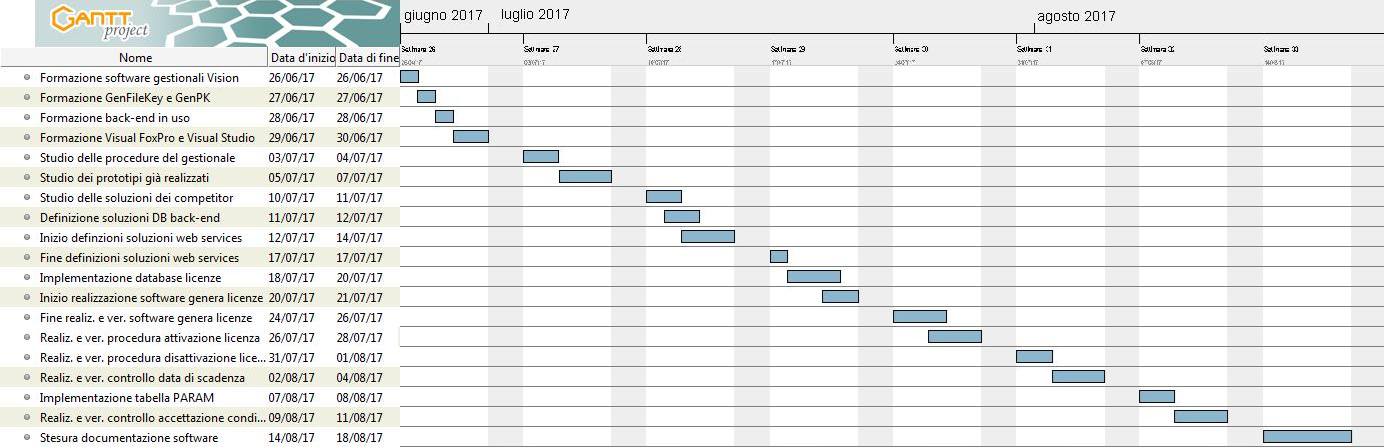
\includegraphics[width=\textwidth]{ganttPrima} 
    \captionof{figure}{Diagramma di Gantt - Pianificazione del lavoro.}
    \label{primastage}
    %\end{minipage}}
    
\end{figure}

\subsection{Resoconto delle attività svolte}
Nella Figura \ref{dopostage} è mostrata la suddivisione delle attività effettivamente svolte. Essa si discosta di molto rispetto quanto pianificato prima di iniziare lo stage. Infatti, grazie a un veloce apprendimento e a una buona progettazione, è stato possibile organizzare il tempo a disposizione per realizzare anche gli obiettivi secondari e facoltativi.
\\

%\rotatebox{90}{\begin{minipage}{0.85\textheight}
\begin{figure}[!h]
\centering
    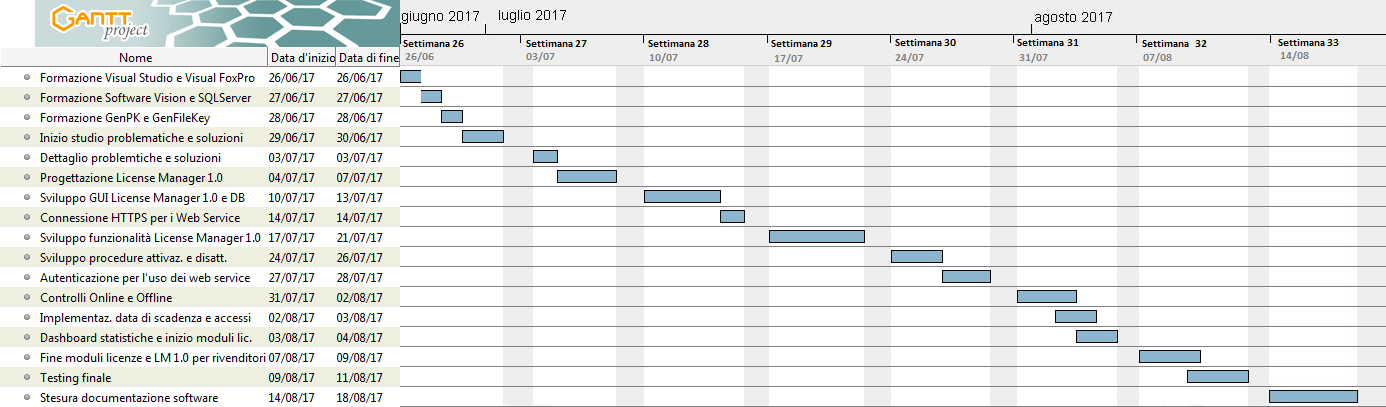
\includegraphics[width=\textwidth]{effettivostage} 
    \captionof{figure}{Diagramma di Gantt - Attività svolte.}
    \label{dopostage}
    %\end{minipage}}
\end{figure}
\newpage

%**************************************************************
\section{Obiettivi e Requisiti}

\subsection{Obiettivi}
Nella fase preliminare dello stage sono stati delineati i seguenti obiettivi, in ordine di importanza. Gli obiettivi sono identificati da un codice così composto:
$$ XXYY $$

dove XX rappresenta la tipologia dell'obiettivo e YY è un numero progressivo utilizzato per differenziare gli obiettivi della stessa categoria.
\\
Le sigle utilizzate sono le seguenti:

\begin{itemize}
\item \textbf{OP:} obiettivo primario;
\item \textbf{OS:} obiettivo secondario;
\item \textbf{OF:} obiettivo facoltativo;
\item \textbf{FO:} obiettivo formativo.
\end{itemize}

Gli obiettivi identificati sono così suddivisi:

\begin{itemize}

\item \textbf{obiettivi primari:}\begin{itemize}
\item OP01: definizione delle strategie risolutive per le problematiche presentate;
\item OP02: implementazione di un sistema di attivazione e disattivazione delle licenze via Web Service;
\item OP03: implementazione di controlli per la validità di una licenza.
\end{itemize}
\item \textbf{obiettivi secondari:}\begin{itemize}
\item OS1: implementazione della data di scadenza di una licenza e relativi controlli.
\end{itemize}
\item \textbf{obiettivi facoltativi:}\begin{itemize}
\item OF01: implementazione delle licenze per moduli;
\item OF02: raccolta dei dati sull’attivazione delle licenze e sul loro utilizzo;
\item OF03: creazione di una dashboard con statistiche e alert sulle licenze in uso, disattivate, e anomalie.
\end{itemize}
\item \textbf{obiettivi formativi:}\begin{itemize}
\item FO01: acquisizione di competenze utili allo sviluppo di software gestionale;
\item FO02: interazione con un team di lavoro aziendale;
\item FO03: ottenimento di capacità decisionali sulle migliori tecnologie da utilizzare in diversi contesti.
\end{itemize}

\end{itemize}

Durante lo svolgimento dello stage, oltre alla creazione e all'attivazione di una licenza, è stato deciso di sviluppare il Software \textit{License Manager 1.0} per gestirne tutti gli aspetti. Dopo aver raggiunto tutti gli obiettivi prefissati, è stato posto come obiettivo ultimo la distribuzione del Software \textit{License Manager 1.0} anche ai rivenditori dell'azienda per concedere loro un certo grado di libertà nella creazione e nella modifica delle licenze. 

\subsection{Requisiti}

In relazione agli obiettivi presentati nel paragrafo precedente sono stati identificati i requisiti riportati in seguito.

\subsubsection{Requisiti OP01}
Per definire una valida strategia risolutiva per le problematiche presentate sono stati identificati i seguenti requisiti:

\begin{itemize}
\item deve essere svolta un'analisi dettagliata del sistema di gestione delle licenze in uso, per analizzarne criticità e debolezze;
\item deve essere affrontato un periodo di formazione sulle tecnologie da utilizzare, per comprenderne al meglio le potenzialità;
\item devono essere delineate e approvate dal tutor aziendale delle soluzioni in grado di risolvere tutte le problematiche presentate.

\end{itemize}

\subsubsection{Requisiti OP02} 
Per implementare un efficiente sistema di attivazione sono stati identificati i seguenti requisiti:
\begin{itemize}
\item deve essere possibile creare un \texttt{Product Key}, secondo le modalità già in uso, da salvare in un Database, eliminando il sistema del file contenente i dati delle licenze condiviso tramite FTP;
\item l'utente finale deve poter inserire all'avvio del \textit{Software Gestionale Vision} il \texttt{Product Key}, ricevuto in fase d'acquisto, relativo alla licenza per lui creata;
\item il \texttt{Product Key} inserito deve essere controllato tramite un metodo di un Web Service, che provvederà a verificare la disponibilità dello stesso e a impostare le informazioni di attivazione della licenza nella tabella \texttt{Licenze} del database \texttt{DBLicenze};
\item il modulo di attivazione, alla risposta del Web Method, deve impostare le chiavi di registro necessarie per il controllo della licenza in modalità Offline;
\item il modulo di attivazione deve essere in grado di riconoscere se la licenza che si sta attivando è già attiva in un altro computer. In caso positivo, tramite una verifica via email, può disattivarla per attivarla sulla macchina corrente;
\item il modulo di attivazione deve essere in grado di riconoscere se la licenza che si sta attivando è attualmente attiva sul computer corrente, riconoscendo le componenti Hardware ma non trovando i riferimenti dell'attivazione della licenza. In caso positivo, tramite una verifica via email, può procedere con la riattivazione;
\item il modulo di attivazione deve essere in grado di bloccare l'attivazione di una licenza in caso di anomalie (ad esempio se una licenza è bloccata);

\end{itemize} 

Per implementare un efficiente sistema di disattivazione sono stati identificati i seguenti requisiti:


\begin{itemize}
\item il modulo di disattivazione deve leggere le chiavi di registro contenenti i riferimenti della licenza, per sapere quale licenza si vuole disattivare;
\item il modulo deve verificare che l'utente sia autorizzato a disattivare la licenza tramite un controllo via email;
\item il modulo deve procedere con la disattivazione invocando un metodo di un Web Service.
\end{itemize}

\subsubsection{Requisiti OP03}

Per implementare un efficiente sistema di controllo della validità di una licenza sono stati identificati i seguenti requisiti:

\begin{itemize}
\item deve essere implementato un controllo, all'avvio del \textit{Software Gestionale Vision} in modalità Online, per verificare che la licenza sia valida in termini di data di scadenza, bloccaggio e componenti Hardware. Il controllo deve essere eseguito tramite Web Service; 
\item deve essere implementato un controllo, all'avvio del \textit{Software Gestionale Vision} in modalità Offline, per verificare che la licenza sia valida in termini di data di scadenza, bloccaggio e componenti Hardware. Il controllo deve essere svolto in locale tramite l'utilizzo di chiavi di registro;
\item deve essere implementato un controllo, che si ripete durante l'esecuzione del \textit{Software Gestionale Vision}, per verificare che la licenza sia in uso su una solo computer per volta, anche in caso di computer identici come macchine virtuali clonate. Il controllo deve essere eseguito tramite Web Service.
\end{itemize}

\subsubsection{Requisiti OS01}

Per correlare a una licenza la data di scadenza, con i relativi controlli, sono stati identificati i seguenti requisiti:

\begin{itemize}
\item tra i campi di un record licenza, salvato nel Database, deve essere presente la data di scadenza;
\item il Software di gestione delle licenze deve essere in grado di impostare e modificare la data di scadenza di una licenza;
\item all'avvio del \textit{Software Gestionale Vision}, sia in modalità Online che Offline, deve essere controllato che la licenza non sia scaduta;
\item all'avvio del \textit{Software Gestionale Vision}, se la licenza è nell'ultimo mese di scadenza il cliente viene avvisato, per dargli la possibilità di estendere la validità.
\end{itemize}

\subsubsection{Requisiti OF01}

Per implementare efficacemente la gestione dei moduli di una licenza sono stati identificati i seguenti requisti:

\begin{itemize}
\item il Software di gestione delle licenze, \textit{License Manager 1.0}, deve dare la possibilità di scegliere e impostare i moduli di una licenza per ogni tipologia;
\item il codice cifrato riepilogativo dei moduli di una licenza deve essere generato come in \textit{GenFileKey}, per assicurare la compatibilità della soluzione;
\item il codice generato deve essere salvato all'interno di un Database, per evitare che sia disponibile all'utente, riducendo i rischi di sicurezza.

\end{itemize}

\subsubsection{Requisiti OF02}

Per raccogliere dati sull'attivazione delle licenze e sul loro utilizzo sono stati identificati i seguenti requisiti:

\begin{itemize}
\item \textit{License Manager 1.0} deve mostrare all'utente il numero di licenze attivate per tipologia;
\item \textit{License Manager 1.0} deve mostrare all'utente il numero di licenze attivate negli ultimi tre anni;
\item \textit{License Manager 1.0} deve permettere agli utenti Admin di visualizzare i dati sulle attivazioni anche in relazione ai rivenditori.
\end{itemize}


\subsubsection{Requisiti OF03}

Per implementare una dashboard con statistiche e alert sulle licenze in uso sono stati identificati i seguenti requisiti:

\begin{itemize}

\item \textit{License Manager 1.0} deve mostrare statistiche utili, come il numero di licenze bloccate, disattivate, scadute o in scadenza;
\item il modulo di avvio del \textit{Software Gestionale Vision} deve tener traccia degli accessi di un utente, registrando i dati in un apposita tabella del Database. \textit{License Manager 1.0} deve mostrare tali accessi;
\item gli accessi multipli di una licenza, ad esempio da diversi \texttt{indirizzi IP} o da diversi \texttt{MAC Address}, devono essere evidenziati da \textit{License Manager 1.0}.

\end{itemize}
\subsubsection{Requisiti FO01}

Per acquisire competenzi utili allo sviluppo di Software gestionale sono stati identificati i seguenti requisiti:

\begin{itemize}
\item è necessario intraprendere un periodo di formazione riguardo il \textit{Software Gestionale Vision};
\item è necessario intraprendere un periodo di formazione riguardo i Software di ausilio al \textit{Software Gestionale Vision}, come \textit{GenPK} e \textit{GenFileKey};
\item è necessario analizzare alcune soluzioni sviluppate dai programmatori dell'azienda in contesti simili.
\end{itemize}

\subsubsection{Requisiti FO02}

Per interagire al meglio con il team di lavoro sono stati identificati i seguenti requisiti:

\begin{itemize}
\item è necessario cercare autonomamente possibili soluzioni prima di chiedere aiuto riguardo qualsiasi problematica;
\item è necessario interrogare il team per decisioni importanti o che potrebbero compromettere le funzionalità di un sistema già in uso;
\item è importante saper valutare la frequenza con cui chiedere aiuto, sia per non disturbare il lavoro altrui sia per non rallentare troppo il proprio.
\end{itemize}

\subsubsection{Requisiti FO03}

Per ottenere capacità decisionali sulle tecnologie da utilizzare in diversi contesti sono stati identificati i seguenti requisiti:

\begin{itemize}
\item è necessario approfondire le possibilità di più tecnologie prima di scegliere quale utilizzare;
\item è necessario effettuare dei test per verificare sommariamente che quanto progettato sia effettivamente realizzabile;
\item è necessario attingere informazioni da più fonti per avere una vista più ampia su quali tecnologie possano essere utili allo scopo. 
\end{itemize}

\subsection{Requisiti \textit{License Manager 1.0}}

I requisiti identificati per \textit{License Manager 1.0} sono i seguenti:

\begin{itemize}
\item il Software deve fornire la possibilità di gestire tutti gli aspetti di una licenza, dalla creazione alla modifica, fino all'eliminazione;
\item il Software deve offire il monitoraggio delle licenze su diversi fronti;
\item il Software deve utilizzare Web Service e Database per svolgere le operazioni;
\item il Software deve essere distribuito ai rivenditori con funzionalità limitate, per preservare la sicurezza dell'azienda.
\end{itemize}
             % Processi
% !TEX encoding = UTF-8
% !TEX TS-program = pdflatex
% !TEX root = ../tesi.tex

%**************************************************************
\chapter{Ambiente di sviluppo}
\label{cap:ambiente-sviluppo}
%**************************************************************

Nel presente capitolo sono illustrate le tecnologie utilizzate per realizzare le soluzioni proposte. Per ogni tecnologia è mostrata una breve descrizione e il suo utilizzo nell'attività di stage.
%**************************************************************
\section{Microsoft Visual Studio 2010}
Visual Studio è un ambiente di sviluppo integrato (\gls{ide}) sviluppato da Microsoft, che supporta diversi tipi di linguaggio, ad esempio C, C++, C\#, F\#, Visual Basic .Net, Html e JavaScript, e che permette la realizzazione di applicazioni, siti web, applicazioni web e servizi web.
\\
Tra le funzioni più interessanti Visual Studio integra la tecnologia \textit{IntelliSense} la quale permette di correggere eventuali errori sintattici (ed alcuni logici) senza compilare l'applicazione, possiede un debugger interno per il rilevamento e la correzione degli errori logici nel codice a runtime, e fornisce diversi strumenti per l'analisi prestazionale.
\\
A differenza dei compilatori classici, quello disponibile col .NET Framework converte il codice sorgente (Visual Basic .NET, C\#, ecc.) in codice IL (Intermediate Language).
IL è un nuovo linguaggio progettato per essere convertito in modo efficiente in codice macchina nativo su differenti tipi di dispositivi; è un linguaggio di livello più basso rispetto a Visual Basic .NET o C\#, ma è a un livello di astrazione più alto rispetto ai linguaggi assembly o linguaggi macchina.
\\
La versione del programma utilizzata durante lo stage è Visual Studio 2010, creato per programmatori che sviluppano per piattaforme Windows e .NET Framework 4.0. Rispetto ai suoi predecessori offre la possibilità di creare applicazioni e servizi Web ASP.NET, in C\# o in VB.NET. È stato distribuito il 12 aprile 2010. 
\\
Il linguaggio di programmazione utilizzato durante lo stage è il C\#.

\subsection{C\#}
Il C\# è un linguaggio di programmazione orientato agli oggetti sviluppato da Microsoft all'interno dell'iniziativa .NET, e successivamente approvato come standard dalla Ecma (ECMA-334) e ISO (norma ISO/IEC 23270).

La sintassi e struttura del C\# prendono spunto da vari linguaggi nati precedentemente, in particolare Delphi, C++, Java e Visual Basic. Il risultato è un linguaggio con meno simbolismo rispetto a C++, meno elementi decorativi rispetto a Java, ma comunque orientato agli oggetti in modo nativo e adatto allo sviluppo di una vasta gamma di Software.

C\# è stato creato da Microsoft specificatamente per la programmazione nel Framework .NET. I suoi tipi di dati "primitivi" hanno una corrispondenza univoca con i tipi .NET e molte delle sue astrazioni, come classi, interfacce, delegati ed eccezioni, sono particolarmente adatte a gestire il .NET framework.


\subsection{Utilizzo nel progetto}

All'interno del progetto l'IDE Microsoft Visual Studio, utilizzando il linguaggio C\#, è stato utilizzato per realizzare tutte le soluzioni, da \textit{License Manager 1.0}, ai Web Service, fino ai moduli da integrare nel \textit{Software Gestionale Vision}. 

\section{Web Service in ASP.NET}

ASP.NET è un insieme di tecnologie di sviluppo di software per il web, commercializzate da Microsoft. Utilizzando queste tecnologie, tramite uno qualsiasi dei linguaggi di alto livello supportati dal framework .NET, come, ad esempio, Visual Basic o C\#, gli sviluppatori possono realizzare applicazioni web e Web Service.
Nel progetto in esame è stato utilizzato il linguaggio C\#{}.

\subsection{Utilizzo nel progetto}

Per la realizzazione delle soluzioni, è stata creata la Web App \texttt{WebLicenseManager} in ASP.NET al solo scopo di contenere i Web Service \texttt{LicenseManagerService}, \texttt{LicenseEmailService} e \texttt{LicenseSecurityService} (illustrati nel capitolo {\hyperref[cap:sviluppo-software]{Web Service e Database}}), senza fornire alcuna funzionalità. Questa metodologia di sviluppo è stata attuata poiché Microsoft Visual Studio 2010 non permette la creazione di Web Service se non contenuti in una Web App.\\
I Web Service creati sono scritti in linguaggio C\#.

\section{Microsoft SQL Server}

Microsoft SQL Server è un \gls{dbms} relazionale sviluppato da Microsoft. Poichè è un Database Server, la sua funzione principale è immagazzinare e ritirare dati in base alle richieste ricevute da altre applicazioni. Esse possono essere eseguite sullo stesso computer o su una qualsiasi macchina connessa alla rete.
\\
Microsoft ha sviluppato molte versioni dello stesso prodotto per soddisfare le diverse richieste degli utenti. Nel progetto in esame è stata utilizzata la versione Microsoft SQL Server 2008 R2, pensato appositamente per contesti aziendali, permettendo una grande capacità di immagazzinamento, e in grado di collaborare perfettamente con Microsoft Visual Studio.

\subsection{Utilizzo nel progetto}

Nel contesto del progetto è stato utilizzato per sviluppare il Database DBLicenze, illustrato nel dettaglio nella sezione \ref{sez:DBLic}.

\section{Microsoft IIS}

Microsoft Internet Information Services, abbreviato in IIS, è un complesso di servizi server Internet per sistemi operativi Microsoft Windows.
IIS è utilizato per ospitare una grande varietà di servizi web, dal Media Streaming alle applicazioni Web. Con IIS Manager è possibile gestire le proprietà delle applicazioni e siti web ospitati, con la possibilità di impostare i protocolli da utilizzare nella connessione, ad esempio FTP, \gls{HTTP} o \gls{HTTPS}. 
La versione utilizzata nel corso dello stage è IIS 7.5, installata su sistema operativo Windows Server 2008 R2.


\subsection{Utilizzo nel progetto}
All'interno del progetto IIS è stato utilizzato per pubblicare l'applicazione Web \texttt{WebLicenseManager} contenente i Web Service sviluppati per soddisfare le richieste dello stage. Tramite IIS Manager è stato possibile impostare la connessione ai Web Service tramite protocollo HTTPS, fornendo un alto livello di sicurezza nella comunicazione Client-Server. La connettività HTTPS è stata stabilità grazie all'utilizzo di un certificato già in possesso dall'azienda.

\section{Microsoft Visual FoxPro}
Visual FoxPro è un linguaggio di programmazione, pubblicato da Microsoft, che integra la programmazione orientata agli oggetti a quella procedurale.

\subsection{Utilizzo nel progetto}
Nell'ambito dello stage è stato necessario apprendere le basi di Visual FoxPro per capire e poter replicare le procedure di generazione del codice cifrato riepilogativo dei moduli di una licenza, poiché scritte in tale linguaggio di programmazione. Le procedure dovevano essere replicate nel modo più preciso possibile per assicurare la corretta decifratura del codice generato tramite il nuovo sistema.              % Kick-Off
% !TEX encoding = UTF-8
% !TEX TS-program = pdflatex
% !TEX root = ../tesi.tex

%**************************************************************
\chapter{Web Service e Database}
\label{cap:sviluppo-software}
%**************************************************************

In questo capitolo sono trattati gli elementi di base delle soluzioni sviluppate. In primo luogo sono illustrati i Web Service responsabili della maggior parte delle operazioni. Successivamente è mostrato il Database di supporto con le principali caratteristiche.


%**************************************************************
\section{Web Service}

Secondo la definizione del (GLOSSARIO)World Wide Web Consortium (W3C), un Web Service è un sistema software progettato per supportare l'interoperabilità tra diversi elaboratori su di una medesima rete.
Questa caratteristica si ottiene associando all'applicazione un'interfaccia Software che espone all'esterno i propri servizi, per mezzo della quale altri sistemi possono interagire con l'applicazione stessa utilizzando le operazioni descritte nell'interfaccia. L'utilizzo delle operazione avviene tramite richieste, nel caso in esame di tipo SOAP (approfondito nella sezione \ref{soap}). I messaggi di richiesta sono formattati secondo lo standard XML, incapsulati e trasportati tramite protocollo HTTPS. 
La connessione implementa il protocollo HTTPS, invece del classico HTTP, per aumentare la sicurezza del sistema, poiché trattandosi di dati riservati un utente malintenzionato vorrebbe poter disturbare la connessione o manometterne i dati trasmessi.\\
Grazie anche all'utilizzo di standard basati su XML, un'architettura basata su Web Service permette ad applicazioni software scritte in diversi linguaggi di programmazione e implementate su diverse piattaforme hardware di utilizzare le funzionalità che essa espone senza difficoltà.
\\Nella Figura \ref{webservice} è mostrato, in modo semplice, il funzionamento di un Web Service.

\begin{figure}[!h] 
    \centering 
    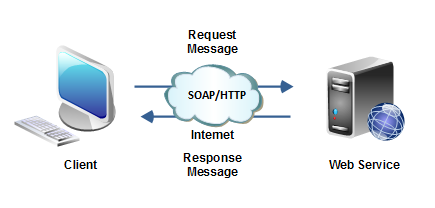
\includegraphics[width=0.60\columnwidth]{web-service} 
    \caption{Funzionamento di un Web Service.}
    \label{webservice}
\end{figure}


Nella realizzazione delle soluzioni sono stati sviluppati tre Web Service,\\ \texttt{LicenseManagerService}, \texttt{LicenseEmailService} e \texttt{LicenseSecurityService}, spiegati nei paragrafi successivi. Ognuno di essi è responsabile di funzionalità ben precise e sono indipendenti tra di loro per fornire un grado più alto di affidabilità ed eliminare le dipendenze.


\subsection{Richieste SOAP}
\label{soap}
SOAP, acronimo di \textit{Simple Object Access Protocol}, è un protocollo per lo scambio di messaggi tra componenti software, nel caso in esame tra Client e Web Service, che avviene per mezzo della sintassi XML. \\
Il protocollo definisce un insieme di regole che il Client deve rispettare per richiedere al server che ospita ed espone il Web Service una determinata operazione.
\\
Un messaggio SOAP è formato da un \texttt{Header} e da un \texttt{Body}:
\begin{itemize}
\item \textbf{Header:} è facoltativo e contiene meta-informazioni, come ad esempio informazioni di sicurezza o parametri per eseguire una procedura;
\item \textbf{Body:} è obbligatorio e contiene il contenuto del messaggio, strutturando secondo (GLOSSARIO)l'XML Schema imposto dal Web Service.
\end{itemize}

Nella Figura \ref{soap} è mostrato un esempio di richiesta e risposta del metodo \texttt{setEmail} del Web Service \texttt{LicenseEmailService}.

\begin{figure}[!h] 
    \centering 
    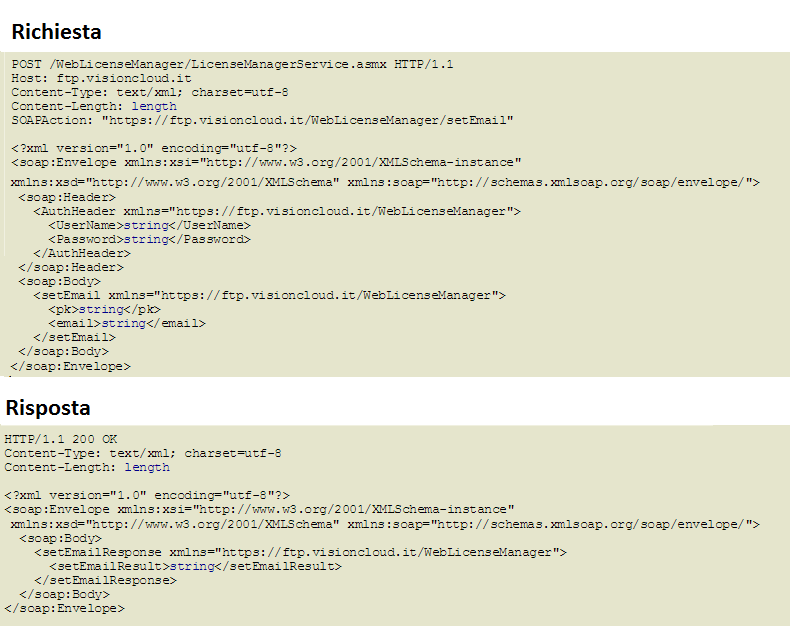
\includegraphics[width=1\columnwidth]{soap} 
    \caption{Esempio di richiesta e risposta SOAP.}
    \label{soap}
\end{figure}

Come si può vedere dalla Figura \ref{soap}, l'\texttt{Header} delle richieste è stato definito in modo da implementare un sistema
di autenticazione, per far sì che i Web Service siano utilizzati esclusivamente da Client autorizzati. Questo argomento è illustrato in dettaglio nel prossimo paragrafo.

\subsection{Autenticazione}
Per preservare la sicurezza dei dati ed evitare che chiunque possa utilizzare i servizi per la gestione delle licenze, è stato implementato un sistema di autenticazione per l'utilizzo dei Web Service. All'arrivo di una richiesta SOAP, i metodi controllano che sia presente l'Header (di norma opzionale), e che esso contenga gli elementi \texttt{UserName} e \texttt{Password}. Una volta verificata la loro esistenza, è invocata una funzione che verifica la validità delle credenziali in essi contenute. Se sono corrette il metodo continua la propria esecuzione, altrimenti ritorna un errore di autenticazione.

\subsection{LicenseManagerService}
\texttt{LicenseManagerService} è il Web Service che si occupa della gestione dei dati delle licenze e degli utenti di \textit{License Manager 1.0}, comunicando con il Database DBLicenze (illustrato nella sezione) per l'archiviazione e il ritiro dei dati. È il Web Service che fornisce più funzionalità, e coi suoi metodi riesce a supportare quasi la totalità delle operazioni richieste da \textit{License Manager 1.0}.\\
Le funzionalità più importanti da esso offerte sono:

\begin{itemize}
\item autenticare un utente per l'utilzzo di \textit{License Manager 1.0};
\item generare un \texttt{Product Key};
\item creare una licenza;
\item bloccare e sbloccare una licenza;
\item modificare la data di scadenza di una licenza;
\item eliminare una licenza;
\item disattivare una licenza;
\item fornire e modificare i moduli di una licenza;
\item restituire la lista delle licenze;
\item restituire la lista degli utenti di \textit{License Manager 1.0};
\item restituire la lista degli accessi al \textit{Software Gestionale Vision};
\item restituire l'insieme delle statistiche riguardanti le licenze;
\item gestire gli utenti di \textit{License Manager 1.0}.

\end{itemize}
 


\subsection{LicenseEmailService}
\texttt{LicenseEmailService} è il Web Service responsabile di gestire le operazioni legate agli indirizzi Email. La funzionalità più importante consiste nel generare un codice casuale e inviarlo tramite mail per verificare l'identità degli utenti e quindi autorizzare le operazioni più importanti. Questa procedura è svolta ad esempio nel momento della disattivazione di una licenza, dove si vuole controllare che l'utente operante sia lo stesso che l'ha attivata, avendo accesso all'indirizzo email inserito in fase di attivazione. L'utente è quindi costretto a inserire lo stesso codice casuale inviato all'indirizzo email associato alla licenza prima di poter continuare con l'operazione.\\
Di seguito sono riportate ulteriori funzionalità che il Web Service offre:
\begin{itemize}
\item restituire l'indirizzo email associato a una licenza;
\item restituire l'indirizzo email associato a un utente di \textit{License Manager 1.0};
\item notificare \textit{VISIONEIMPRESA s.r.l.} alla creazione di una licenza da parte di un rivenditore;
 \item notificare \textit{VISIONEIMPRESA s.r.l.} alla modifica di una licenza da parte di un rivenditore;
 \item inviare le credenziali di primo accesso a un nuovo utente di \textit{License Manager 1.0};
 \item inviare il \texttt{Product Key} da usare per una nuova attivazione in seguito alla disattivazione di una licenza.
\end{itemize}

\subsection{LicenseSecurityService}
\texttt{LicenseSecurityService} è il Web Service responsabile dei controlli da effettuare su una licenza e dell'area relativa alla sicurezza delle soluzioni sviluppate. La funzionalità più importante consiste nel verificare la validità di una licenza in termini di bloccaggio, data di scadenza e componente Hardware. A un esito positivo il metodo responsabile ritorna una stringa contenente le informazioni da utilizzare per il controllo della validità di una licenza in modalità Offline. Il funzionamento dettagliato è affrontato nella sezione \ref{off}.
Per assicurare l'integrità dei messaggi scambiati col server, ove necessario, è utilizzato un sistema di cifratura a chiave pubblica, ad esempio per firmare i messaggi inviati dal server.\\
Le altre funzionalità che il Web Service offre sono:
\begin{itemize}
\item eseguire il controllo di una licenza durante l'esecuzione del \textit{Software Gestionale Vision}, affrontato nella sezione \ref{uniqueid};
\item restituire la chiave pubblica del server;
\item firmare digitalmente un messaggio con la chiave privata del server.

\end{itemize}


%**************************************************************
\section{Database}
\label{sez:DBLic}
Per l'archiviazione dei dati è utilizzato il Database relazionale DBLicenze, creato con SQLServer di Microsoft. L'ottenimento dei dati, per questioni di sicurezza, è affidato ai soli Web Service. Qualsiasi soluzione sviluppata deve affidarsi ai Web Service per interrogare il Database, aumentando il grado di affidabilità e riservatezza. L'utilizzo di un Database, in sostituzione al file condiviso tramite FTP, assicura maggiore consistenza dei dati, uso contemporaneo delle risorse grazie all'atomicità delle transazioni, controllo degli accessi, facilità nel reperimento dei dati e stabilità del sistema.


\subsection{DBLicenze}
Per raccogliere i dati relativi alla gestione e al controllo delle licenze è stato utilizzato un unico Database: \texttt{DBLicenze}. In seguito sono illustrate le tabelle che compongono il Database.

\subsubsection{Licenze}
È la tabella fondamentale contenente le licenze del \textit{Software Gestionale Vision}. \\Le informazioni in essa contenute, per ogni licenza, sono le seguenti:

\begin{itemize}
\item Product Key;
\item Serial Number;
\item tipologia;
\item componente Hardware associata alla licenza. Essa è espressa tramite una chiave esterna riferita alla tabella HWComponent;
\item eventuale blocco della licenza;
\item data di attivazione;
\item data di scadenza;
\item data di ultima attivazione;
\item numero di reinstallazioni;
\item data di ultimo accesso;
\item cliente;
\item email associata;
\item codice cifrato dei moduli;
\item codice dell'utente creatore;
\item autore del blocco, se presente;
\item data di creazione.
\end{itemize}

\subsubsection{Utenti}

Contiene gli utenti del Software \textit{License Manager 1.0}.\\ Le informazioni, per ogni utente, sono:

\begin{itemize}
\item username;
\item hash della password in (glossario)SHA256;
\item essere admin;
\item poter resettare la propria password;
\item codice utente (o codice rivenditore);
\item email associata all'utente.
\end{itemize} 

\subsubsection{HWComponent}

Contiene i dettagli dei computer che hanno o hanno avuto una licenza del \textit{Software Gestionale Vision} installata su di essi. \\Per ogni computer, le informazioni salvate sono:

\begin{itemize}
\item diverse componenti Hardware, non specificate per motivi di sicurezza;
\item Product Key della licenza associata;
\item data di attivazione della licenza;
\item data di disattivazione della licenza.
\end{itemize}

Alla disattivazione di una licenza il record relativo al computer da dissociare non è eliminato, ma rimane nella tabella impostando la data di disattivazione. In questo modo l'azienda è in grado di avere una panoramica completa sui PC in cui una licenza è stata installata, potendo notare possibili anomalie (ad esempio il ripetersi di installazioni sulle stesse macchine). 

\subsubsection{LicenseTransmittedID}

Contiene gli UniqueID utilizzati per il controllo durante l’esecuzione del Software Gestionale Vision (riferirsi alla sezione \ref{uniqueid} per maggiori dettagli). \\Ogni record possiede le seguenti informazioni:

\begin{itemize}
\item Product Key della licenza a cui è associato l'UniqueID;
\item UniqueID utilizzato per il controllo;
\item contatore delle risincronizzazioni effettuate;
\item eventuale permesso di risincronizzazione;
\item timestamp utilizzato per resettare il contatore delle risincronizzazioni ogni mese.
\end{itemize}

Il contatore delle risincronizzazioni è utilizzato per monitorare quante volte l'UniqueID non viene trovato sul PC di cui verificare la validità della licenza. Esso può non essere trovato ad esempio per un eliminazione involontaria dei file responsabili al controllo. Il numero di risincronizzazioni permesse è tre ogni mese, in seguito l'azienda è informata dell'anomalia.


\subsubsection{EmailCodice}

Contiene i codici inviati via Email per controllare l’effettivo possesso dell’indirizzo email da parte degli utenti del \textit{Software Gestionale Vision}.
\\Ogni record possiede le seguenti informazioni:

\begin{itemize}
\item ID del codice da verificare;
\item indirizzo email a cui è associato il codice;
\item codice da verificare;
\item timestamp per rendere inutilizzabile il codice dopo 10 minuti.
\end{itemize}

Ogni indirizzo email può avere più codici in attesa di verifica (situazione causata dalla non ricezione delle mail che li contenevano), ma solo il più recente è ritenuto valido e utilizzato per il controllo. Inoltre, i codici generati da più di 10 minuti sono eliminati per questioni di sicurezza.

\subsubsection{LogAccessi}

Contiene gli accessi al \textit{Software Gestionale Vision}.
\\Ogni accesso ha le seguenti caratteristiche:

\begin{itemize}
\item ID dell'accesso;
\item Product Key della licenza di cui si registra l'accesso;
\item indirizzo IP dell'accesso;
\item MAC Address della scheda di rete del computer da cui si è effettuato l'accesso;
\item data dell'accesso;
\item codice utente associato alla licenza di cui si registra l'accesso.
\end{itemize}

Tra le informazioni è salvato anche il codice utente associato alla licenza per poter avere la lista degli accessi filtrabile per i diversi rifornitori.

\subsubsection{StoricoStatiLicenze}

Contiene gli stati passati di una licenza. Ogni stato è stato creato in seguito a una modifica. Lo stato attuale di una licenza è presente nella tabella Licenze.
\\Ogni stato è caratterizzato dalle informazioni variabili di una licenza, ed ha quindi le seguenti informazioni:

\begin{itemize}
\item ID dello stato;
\item componente Hardware;
\item eventuale blocco;
\item data di scadenza;
\item cliente;
\item email;
\item codice cifrato dei moduli;
\item codice utente;
\item data di fine validità dello stato.
\end{itemize}

Disponendo di una tabella contenente gli stati di tutte le licenze antecedenti le modifiche, l'azienda è in grado di avere una panoramica su tutto lo storico delle proprie licenze, evitando ad esempio equivoci con i rivenditori.             % Concept Preview
% !TEX encoding = UTF-8
% !TEX TS-program = pdflatex
% !TEX root = ../tesi.tex

%**************************************************************
\chapter{\textit{License Manager 1.0}}
\label{cap:license-manager}
%**************************************************************

\textit{License Manager 1.0} nasce con lo scopo di creare nuove licenze, eliminando \textit{GenPK} e le problematiche ad esso correlato. Nel corso dello stage, con il delinearsi di nuovi obiettivi, il programma è stato ampliato per poter gestire la maggior parte degli aspetti di una licenza, incluso il monitoraggio. Le funzionalità del Software sono svolte tramite chiamate a Web Service, i quali utilizzano il Database \texttt{DBLicenze} per il salvataggio dei dati.
\\
Inizialmente pensato per un uso interno all'azienda, grazie alle molteplici funzionalità che esso offriva, è stato deciso di distribuire il Software anche ai rivenditori, concedendo loro una maggior capacità operativa.
I rivenditori, per la sicurezza dell'azienda, possono usufruire di operazioni limitate, e le modifiche più rilevanti sono comunicate a \textit{VISIONEIMPRESA} tramite mail.


%**************************************************************
\section{Scopo del prodotto}

Con \textit{License Manager 1.0} si vuole racchiudere in un unico programma la possibilità di gestire completamente le licenze del \textit{Software Gestionale Vision}, dalla creazione all'eliminazione, con la possibilità di effettuare modifiche, ricevere statistiche e monitorare lo stato delle licenze per notare possibili anomalie. 

%**************************************************************

\section{Tipologie di utenti}

\textit{License Manager 1.0} gestisce due tipologie di utente, \textit{Admin} e \textit{Guest}.

\begin{itemize}
\item \textbf{\textit{Admin}}: ha a disposizione tutte le funzionalità senza limitazioni, ed è ideato per i soli membri dell’azienda. Un utente di questo tipo può visualizzare e modificare tutte le licenze, indipendentemente da chi le abbia create;

\item \textbf{\textit{Guest}}: ha a disposizione tutte le funzionalità ma con alcune limitazioni. Questo tipo di utente è creato per ogni rivenditore, in modo che esso possa gestire solo le licenze da esso vendute, senza interferire con le licenze create dall’azienda o da altri rivenditori. Ad ogni \textit{Guest} è associato un \texttt{Codice Utente}, ossia un codice definito per lo specifico rivenditore, e più \textit{Guest} possono avere lo stesso \texttt{Codice Utente}, poiché un rivenditore potrebbe voler affidare la gestione delle proprie licenze ad utenti diversi.
\end{itemize}


%**************************************************************
\section{Autenticazione}
Poiché il programma si propone di gestire diverse tipologie di utenti è stato implementato un sistema di autenticazione. In Figura \ref{auth} è mostrato il Form di autenticazione, visibile all'avvio del programma.

\begin{figure}[!h] 
    \centering 
    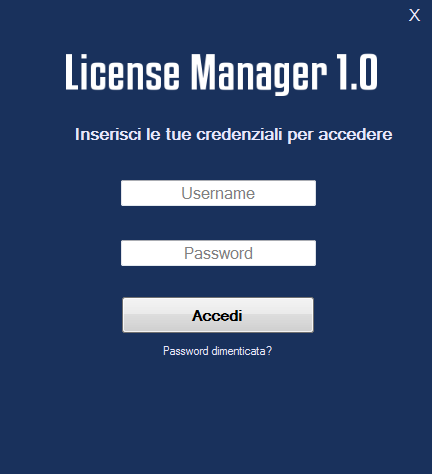
\includegraphics[width=0.5\columnwidth]{LicenseManager/auth} 
    \caption{License Manager 1.0 - Form di autenticazione}
    \label{auth}
\end{figure}

L’utente, per accedere, deve inserire il proprio \texttt{Username} e la \texttt{Password}, e cliccare su "Accedi".\\
Solo gli \textit{Admin} possono creare gli utenti, scegliendone l’username, un indirizzo email da associare, e nel caso l’utente sia destinato a un rivenditore è data la possibilità di sceglierne il \texttt{Codice Utente} (o codice rivenditore).
Un utente che ha dimenticato la password è costretto a contattare un \textit{Admin} per chiederne il reset. Se l’\textit{Admin} concede il reset della password, inserendo l’\texttt{Username} e cliccando su "Password dimenticata?" è possibile impostare una nuova Password.\\
Per maggiori dettagli sulla gestione degli utenti si rimanda alla sezione X.X9 “Amministra utenti”.
\newpage


%**************************************************************
\section{Struttura generale del Software}
Dopo l'autenticazione, il programma si mostra come in Figura \ref{primscher}.

\begin{figure}[!h] 
    \centering 
    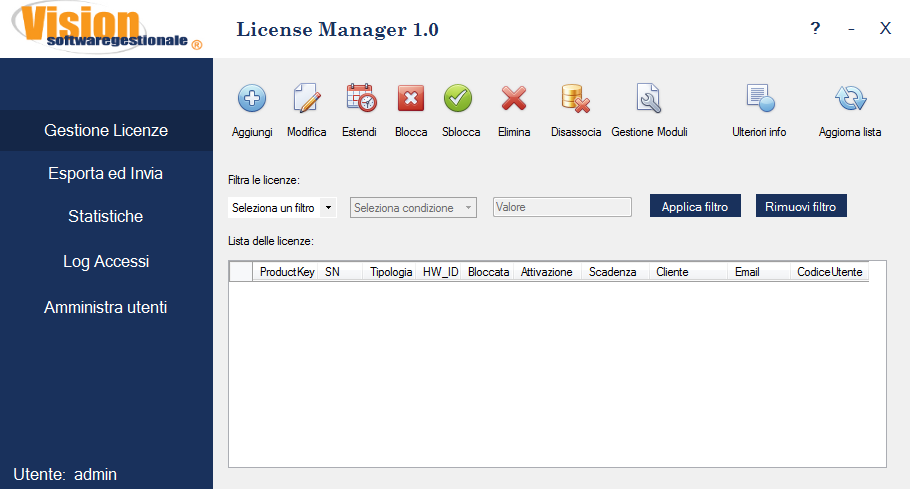
\includegraphics[width=1\columnwidth]{LicenseManager/primaSchermata} 
    \caption{License Manager 1.0 - Prima schermata all'avvio}
    \label{primscher}
\end{figure}

È presente un menu laterale, sulla sinistra, che permette la navigazione tra le diverse sezioni del programma:

\begin{itemize}
\item \textbf{Gestione Licenze:} Sono presenti tutte le funzionalità che permettono di gestire le licenze, dalla creazione all’eliminazione;
\item \textbf{Esporta ed Invia:} Sono presenti funzionalità che permettono di creare un file riepilogativo della licenza o esportare in un file Excel il riepilogo di alcuni dati;
\item \textbf{Statistiche:} Sono presenti alcune statistiche delle licenze visibili all’utente. Un \textit{Admin} può visualizzare le statistiche di tutte le licenze o di quelle associate a un rivenditore, mentre un \textit{Guest} può visualizzare le solo le statistiche delle licenze ad esso associate;
\item \textbf{Log Accessi:} Permette di visualizzare gli accessi al \textit{Software Gestionale Vision} delle proprie licenze, per monitorare eventuali anomalie;
\item \textbf{Amministra utenti:} Sezione visibile solo agli amministratori, dove è possibile gestire gli utenti del programma.

\end{itemize}

In basso a sinistra è riportato l’utente con cui si è acceduti.
\\
Tutte le sezioni saranno spiegate nel dettaglio nei prossimi paragrafi.

%**************************************************************
\newpage
\section{Gestione Licenze}
La sezione "Gestione Licenze" è la prima a mostrarsi dopo l'autenticazione. \\ In Figura \ref{gestLic} è possibile vedere una situazione esempio della sezione.

\begin{figure}[!h] 
    \centering 
    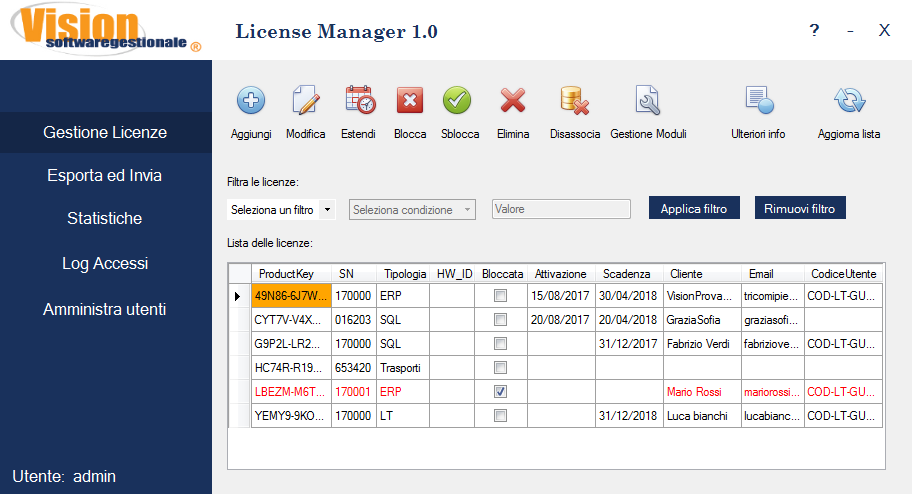
\includegraphics[width=0.9\columnwidth]{LicenseManager/gestLic} 
    \caption{License Manager 1.0 - Gestione Licenze}
\label{gestLic}
\end{figure}

Nella sezione “Gestione Licenze“ è possibile gestire tutti gli aspetti delle licenze.
Nello specifico le operazioni permesse, nell'ordine, sono:
\begin{itemize}
\item \textbf{Aggiungi:} permette di creare una nuova licenza;
\item \textbf{Modifica:} permette di modificare diversi aspetti di una licenza;
\item \textbf{Estendi:} permette di posticipare la data di scadenza;
\item \textbf{Blocca:} permette di bloccare una licenza;
\item \textbf{Sblocca:} permette di sbloccare una licenza;
\item \textbf{Elimina:} permette di eliminare una licenza;
\item \textbf{Disassocia:} permette di dissociare una licenza dalla propria componente Hardware;
\item \textbf{Gestione Moduli:} permette di gestire i moduli della licenza;
\item \textbf{Ulteriori Info:} fornisce ulteriori informazioni sulla licenza;
\item \textbf{Aggiorna lista:} permette di aggiornare la lista delle licenze;
\item \textbf{Applica filtro:} permette di filtrare le licenze in base a determinate condizioni;
\item \textbf{Rimuovi filtro:} rimuove il filtro precedentemente selezionato.
\end{itemize} 
Nella parte alta della schermata sono presenti le funzionalità, mentre nella parte bassa è mostrata la lista delle licenze visibili all’utente.
\\
Un \textit{Admin} può visualizzare tutte le licenze, ed eventualmente filtrarle per \texttt{Codice Utente} per visualizzare le licenze assegnate a un rivenditore.
\\
Un \textit{Guest} (o rivenditore), può visualizzare solo le licenze con \texttt{Codice Utente} uguale al proprio.
\\

In generale, prima che avvenga una modifica a una licenza (o l'eliminazione), tramite l'utilizzo del Web Service \texttt{LicenseManagerService}, è salvato il suo stato attuale nella tabella \texttt{StoricoStatiLicenze} per avere lo storico completo di tutte le licenze. Inoltre, se la modifica è stata apportata da un \textit{Guest}, essa è notificata all'azienda tramite l'utilizzo del Web Service \textit{LicenseEmailService} per mantenere l'azienda informata sullo stato di tutte le licenze. 
\\Nei paragrafi successivi sono mostrate nel dettaglio tutte le funzionalità. 

\subsection{Aggiungi}
La funzione “Aggiungi” permette di creare una nuova licenza. Il metodo di creazione differisce per gli utenti Admin e gli utenti Guest. Cliccando sul pulsante si apre una nuova finestra, dove è possibile inserire i dati di una licenza. La finestra è riportata nella Figura \ref{crealic}.

\begin{figure}[!h] 
    \centering 
    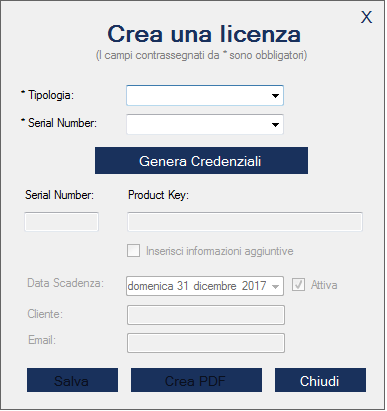
\includegraphics[width=0.55\columnwidth]{LicenseManager/creaLicenza} 
    \caption{Finestra Aggiungi - Gestione Licenze}
    \label{crealic}
\end{figure}

Per creare una licenza è necessario innanzitutto valorizzare i campi obbligatori, ovvero \texttt{Tipologia} e \texttt{Serial Number}. 
\begin{itemize}

\item \textbf{Tipologia:} Identifica quale licenza si sta creando, e i valori possibili sono SQL, LT, ERP o Trasporti. 
\item \textbf{Serial Number:} Numero di sei cifre che identifica in modo univoco, per tipologia, una licenza. Uno stesso Serial Number è permesso per diverse tipologie. La scelta del Serial Number differisce da Admin e Guest.  
\begin{itemize}

\item	\textbf{Admin:} Può scegliere tra un \texttt{Serial Number}:
\begin{itemize}
\item \textbf{Manuale:} scelto arbitrariamente;
\item \textbf{Casuale:} generato casualmente dal programma;
\item \textbf{Prime due cifre per l'anno:} le prime due cifre sono le ultime due cifre dell'anno corrente, mentre le restanti quattro identificano il punto di partenza da cui cercare un \texttt{Serial Number} libero.
\end{itemize}
\item	\textbf{Guest:} Può creare solo un \texttt{Serial Number} di tipologia “Prime due cifre per l’anno”.
\end{itemize}

\end{itemize}	

Dopo aver scelto Tipologia e Serial Number è necessario cliccare su "Genera Credenziali" per poter continuare con la creazione della licenza. Cliccando su questo pulsante è invocato un metodo del Web Service \texttt{LicenseManagerService} che produrrà un \texttt{Serial Number} compatibile con la scelta effettuata e un \texttt{Product Key} che identifica univocamente una licenza, indipendentemente dalla tipologia. Qualora il Serial Number scelto in caso di selezione "Manuale" o "Casuale" fosse già in uso, sarà comunicato che non è possibile utilizzare tali valori ed è necessario sceglierne degli altri. In caso di scelta "Prime due cifre per l’anno" il \texttt{Serial Number} prodotto sarà il primo libero disponibile a partire dal numero a quattro cifre scelto. Dopo la creazione delle credenziali il pulsante "Salva" si attiverà e sarà possibile salvare la licenza, come si evince dalla Figura \ref{salva}.

 \begin{figure}[!h] 
    \centering 
    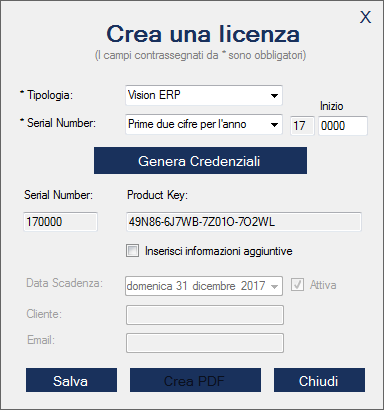
\includegraphics[width=0.55\columnwidth]{LicenseManager/salva} 
    \caption{License Manager 1.0 - Salvataggio di una licenza appena creata}
\label{salva}
\end{figure}

Prima di procedere con il salvataggio è possibile definire delle informazioni aggiuntive della licenza, come la data di scadenza, il cliente cui è destinata e l’email da associare alla licenza. La data di scadenza può essere attivata o disattivata grazie alla checkbox "Attiva" a lato del selettore della data. Nel caso di inserimento di informazioni aggiuntive è possibile anche creare direttamente il PDF contenente i dettagli della licenza da spedire al cliente. Cliccando su "Crea PDF" sarà prima chiesto di salvare la licenza.
\\Nella Figura \ref{pdf} è mostrato l'inserimento delle informazioni aggiuntive con la creazione diretta del file PDF.


\begin{figure}[!h] 
    \centering 
    \includegraphics[width=0.9\columnwidth]{LicenseManager/creaPDFInfoAggi} 
    \caption{License Manager 1.0 - Informazioni aggiuntive e creazione file PDF}
\label{pdf}
\end{figure}

Una licenza creata da un \textit{Guest} avrà come \texttt{Codice Utente} il suo codice, mentre se è creata da un \textit{Admin} esso sarà inizialmente nullo e potrà essere impostato in seguito attraverso la funzione "Modifica".
\\
L’esecuzione del salvataggio cambia a seconda di una creazione da parte di un \textit{Admin} o di un \textit{Guest}.
Solo se a creare la licenza è stato un \textit{Guest} viene prima notificata via mail l'azienda \textit{VISIONEIMPRESA}, attraverso l'utilizzo del Web Service \texttt{LicenseEmailService}, e poi si procede al salvataggio della licenza tramite l'utilizzo del Web Service \texttt{LicenseManagerService}. Se la notifica dovesse fallire l’operazione di salvataggio non viene eseguita, in quanto potrebbe sfuggire la creazione di una licenza. Se un errore dovesse incorrere durante il salvataggio sarà inviata una seconda mail per avvertire che la mail di creazione inviata in precedenza potrebbe essere errata.\\
Se a creare la licenza è un \textit{Admin} l'azienda non viene notificata.
\\
Infine, se la creazione è andata a buon fine, è mostrato un messaggio che lo conferma e la schermata di creazione viene chiusa. Nella lista delle licenze apparirà quindi la nuova licenza appena creata, come si può vedere nella Figura \ref{nuova}.

\begin{figure}[!h] 
    \centering 
    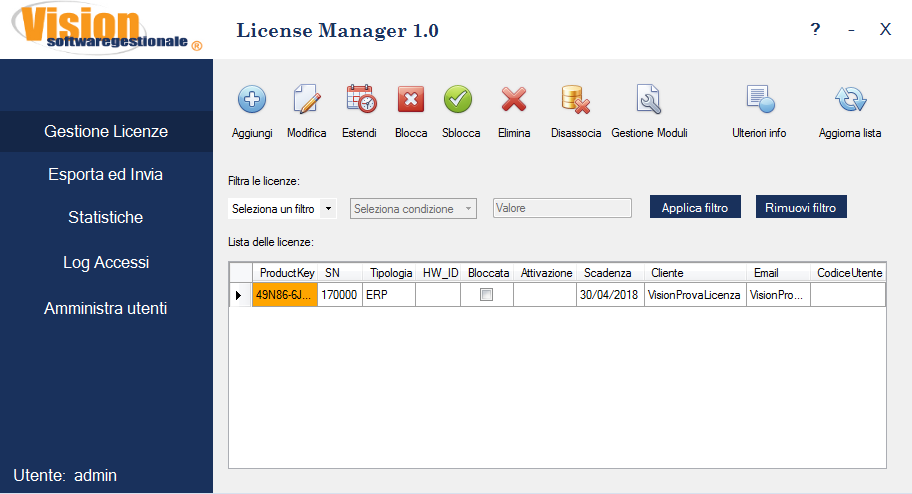
\includegraphics[width=0.85\columnwidth]{LicenseManager/nuovalicenza} 
    \caption{License Manager 1.0 - Aggiunta alla lista di una licenza appena creata}
\label{nuova}
\end{figure}


\subsection{Modifica}

La funzione "Modifica" permette di modificare i dati non immutabili di una licenza:
\begin{itemize}
\item \textbf{Data di scadenza:} data di scadenza di una licenza, può anche essere rimossa;
\item \textbf{Cliente:} nome del cliente, utilizzato per comodità per riferirsi a una licenza;
\item \textbf{Email:} indirizzo email associato alla licenza. Tramite l’indirizzo email il cliente può disattivare e riattivare la propria licenza senza che sia necessario contattare l’azienda. Per questo motivo ai \textit{Guest} non è data la possibilità di modificare l’email decisa dai clienti in fase di attivazione;
\item \textbf{Codice Utente:} codice del rifornitore cui è assegnata la licenza. Un rifornitore sarà in grado di vedere solo le licenze con il codice utente uguale a quello a lui assegnato. Per questo motivo anche il \texttt{Codice Utente} non può essere modificato dai rifornitori.
Gli \textit{Admin}, invece, possono vedere tutte le licenze e modificarne il \texttt{Codice Utente}, a meno che la licenza non sia impostata come "Licenza ad uso interno non rivendibile". Riferirsi alla sezione x.x per ulteriori informazioni.
\end{itemize} 

In Figura \ref{modifica} è mostrata la schermata di modifica.

\begin{figure}[!h] 
    \centering 
    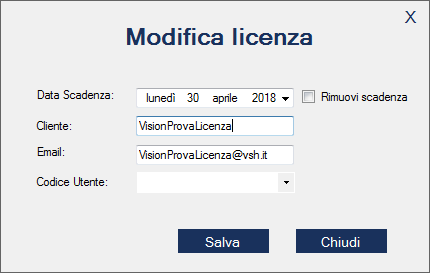
\includegraphics[width=0.6\columnwidth]{LicenseManager/modifica} 
    \caption{License Manager 1.0 - Modifica di una licenza}
\label{modifica}
\end{figure}

\newpage
\subsection{Estendi}
La funzione "Estendi" permette di modificare velocemente la data di scadenza, scegliendone una nuova o indicando il numero di mesi di cui si vuole estendere la licenza.
Il Form relativo è mostrato in Figura \ref{estendi}.

\begin{figure}[!h] 
    \centering 
    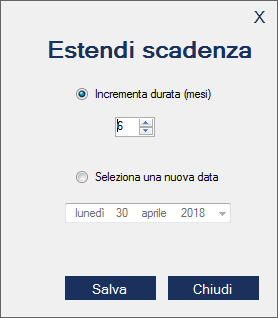
\includegraphics[width=0.45\columnwidth]{LicenseManager/Estendi} 
    \caption{License Manager 1.0 - Estensione del periodo di validità di una licenza}
\label{estendi}
\end{figure}

\subsection{Blocca}

La funzione "Blocca" permette di bloccare una licenza. All’accesso del \textit{Software Gestionale Vision} se la licenza è bloccata viene mostrato un messaggio d’errore e non è permesso l’utilizzo.
Le licenze bloccate sono mostrate in rosso nella lista delle licenze, cosi come le licenze scadute.
È possibile anche bloccare più licenze in una volta selezionandole dalla lista.
\\
Nella Figura \ref{block} si può vedere un esempio di licenza bloccata.
\begin{figure}[!h] 
    \centering 
    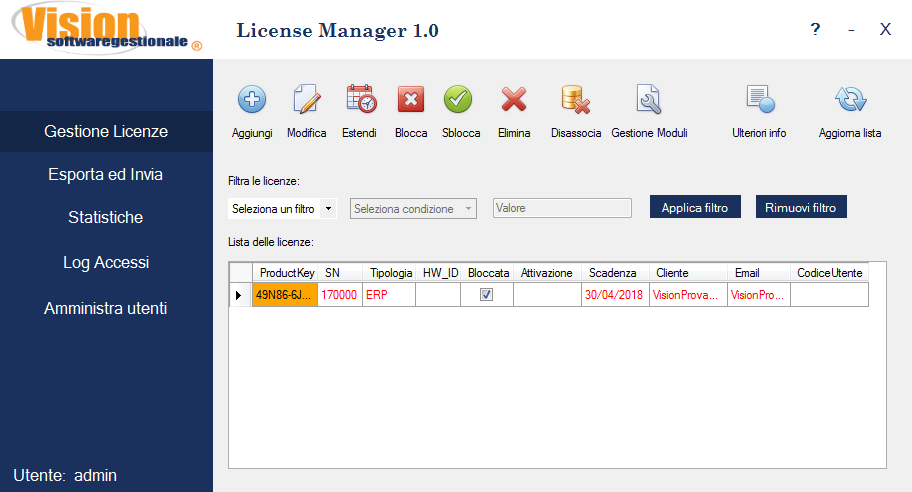
\includegraphics[width=0.8\columnwidth]{LicenseManager/bloccate} 
    \caption{License Manager 1.0 - Licenza bloccata}
\label{block}
\end{figure}

\subsection{Sblocca}
La funzione "Sblocca" permette di sbloccare una licenza bloccata in precedenza.
I rivenditori possono sbloccare solo le licenze da loro bloccate, per evitare di rimuovere i blocchi imposti dagli \textit{Admin}.\\
Come si vede nella Figura \ref{sblocca}, accedendo con un utente di tipo \textit{Guest} (in questo caso "ProvaLT"), non è possibile sbloccare una licenza bloccata da un \textit{Admin}.

\begin{figure}[!h] 
    \centering 
    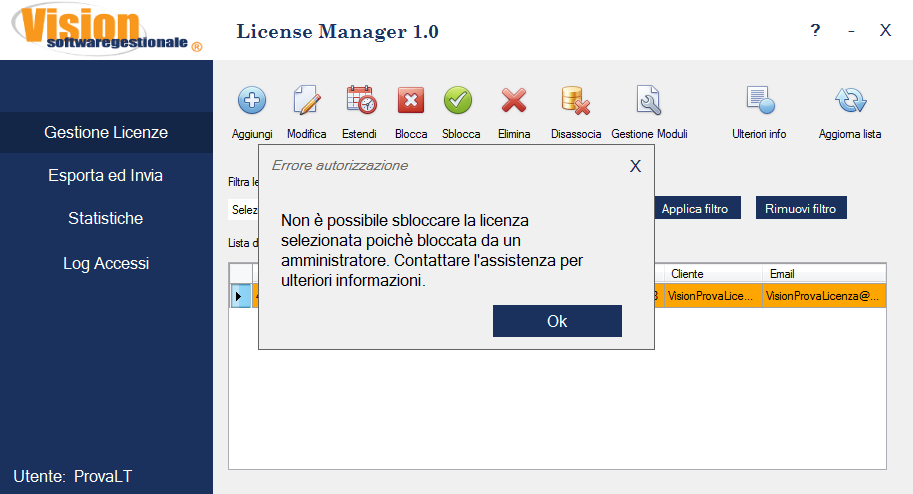
\includegraphics[width=0.8\columnwidth]{LicenseManager/sblocca} 
    \caption{License Manager 1.0 - Sblocco di una licenza}
\label{sblocca}
\end{figure}

\subsection{Elimina}
La funzione “Elimina” permette di rimuovere una licenza, tuttavia agisce in modo diverso se a richiedere l'eliminazione è un \textit{Admin} o un \textit{Guest}. Mentre per l’\textit{Admin} l’eliminazione è sempre concessa, un \textit{Guest} può eliminare la licenza solo se non è mai stata attivata o se non sono ancora stati definiti i moduli per quella licenza.\\
Nella Figura \ref{elim} l’utente \textit{Guest} "ProvaLT", tentando l’eliminazione dopo che i moduli della licenza sono stati definiti, viene avvisato e l’eliminazione non avviene.

\begin{figure}[!h] 
    \centering 
    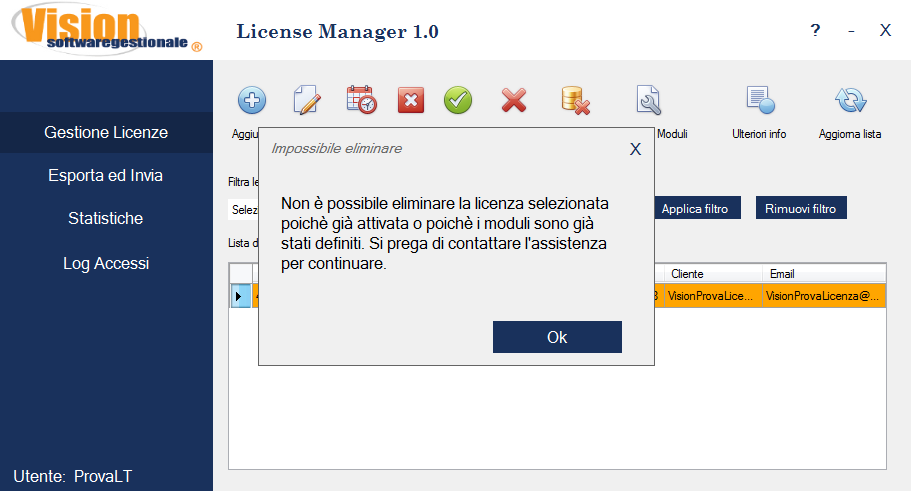
\includegraphics[width=0.8\columnwidth]{LicenseManager/elimin} 
    \caption{License Manager 1.0 - Eliminazione di una licenza}
\label{elim}
\end{figure}

\subsection{Disassocia}

La funzione "Disassocia" permette di dissociare una licenza dalla sua componente Hardware, utilizzata per verificare che la licenza sia utilizzata in un solo computer per volta. 
Dissociando una licenza dalla sua componente Hardware se ne permette la reinstallazione in una nuova macchina, mentre su quella attuale all’avvio del \textit{Software Gestionale Vision} risulterà che la licenza non è più associata a quel dispositivo.

\subsection{Gestione Moduli}

La funzione "Gestione Moduli" permette di selezionare quali moduli associare a una licenza. Sia \textit{Admin} che \textit{Guest} possono selezionare i moduli, ma con delle differenze: gli \textit{Admin} possono modificare i moduli un qualsiasi numero di volte, mentre i \textit{Guest} possono impostarli solo una volta dopo la creazione, dopodiché la modifica non sarà più permessa. Se i moduli sono già stati definiti da un \textit{Admin} allora il \textit{Guest} non potrà modificarli.
Cliccando su "Gestione Moduli", in base alla tipologia della licenza, si apre una nuova finestra che si presenta come nella Figura \ref{gest}.

\begin{figure}[!h] 
    \centering 
    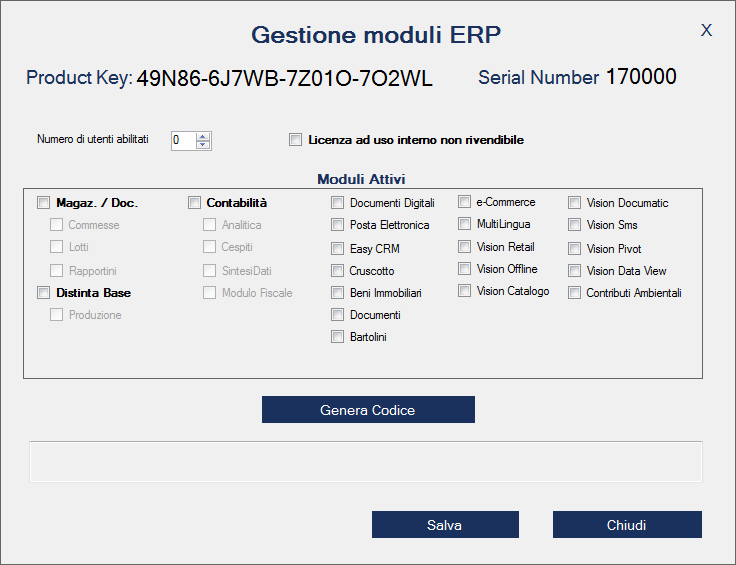
\includegraphics[width=1\columnwidth]{LicenseManager/gestmoduli} 
    \caption{License Manager 1.0 - Gestione dei moduli di una licenza}
\label{gest}
\end{figure}

Da qui è possibile selezionare il numero di utenti abilitati e i moduli da attivare. Inoltre a un \textit{Admin} è permesso impostare la licenza come "Licenza ad uso interno non rivendibile", che selezionerà automaticamente tutti i moduli e non potrà essere associata a un codice utente.\\
Una volta scelti i moduli è necessario cliccare su "Genera Codice" per generare il codice riassuntivo dei moduli scelti, che viene creato come dal programma \textit{GenFileKey}. Il codice generato è quindi il codice cifrato che in precedenza veniva salvato nei file di configurazione ".HWK".  Dopo aver generato il codice, la situazione si presenta come nella Figura \ref{codcreat}.

\begin{figure}[!h] 
    \centering 
    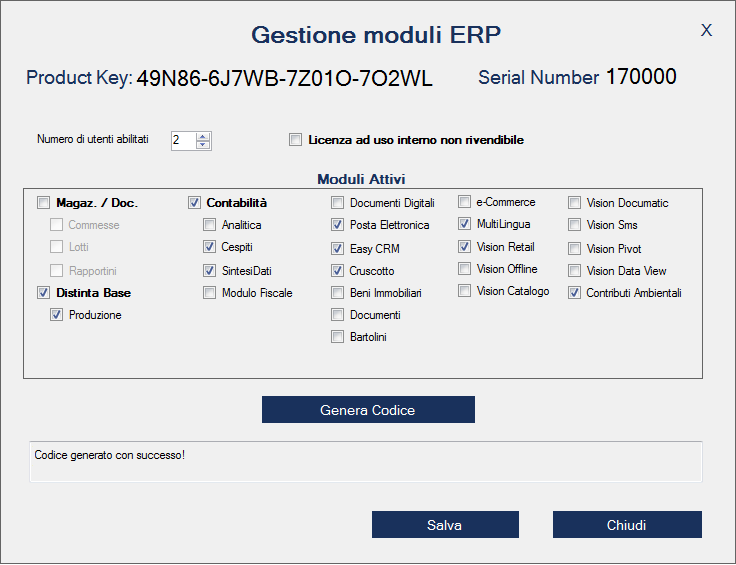
\includegraphics[width=1\columnwidth]{LicenseManager/codgen} 
    \caption{License Manager 1.0 - Creazione del codice moduli}
\label{codcreat}
\end{figure}

Nel caso a generare il codice fosse un \textit{Admin}, nel riquadro al posto di "Codice generato con successo!" sarebbe mostrato il codice generato.
\\
A questo punto è necessario salvare con il pulsante "Salva" per rendere effettive le modifiche.
Un \textit{Admin} può definire più volte i moduli nella stessa schermata, ma dopo aver salvato la prima volta è necessario rigenerare il codice per poter salvare nuovamente.\\
L’esecuzione del salvataggio cambia a seconda della definizione dei moduli da parte di un \textit{Admin} o di un \textit{Guest}.
Solo se a creare la licenza è stato un \textit{Guest} viene prima notificata via mail l'azienda \textit{VISIONEIMPRESA}, attraverso l'utilizzo del Web Service \texttt{LicenseEmailService}, e poi si procede al salvataggio dei moduli tramite l'utilizzo del Web Service \texttt{LicenseManagerService}. Se la notifica dovesse fallire l’operazione di salvataggio non viene eseguita, in quanto potrebbe sfuggire la definizione dei moduli, operazione fondamentale per una corretta fatturazione della licenza. Se un errore dovesse incorrere durante il salvataggio sarà inviata una seconda mail per avvertire che la mail inviata in precedenza potrebbe essere errata.
Una mail riepilogativa dei moduli è inviata anche all'indirizzo email associato all'utente che sta definendo i moduli.

\newpage

\subsection{Ulteriori Info}
La funzione "Ulteriori Info" permette di visualizzare delle informazioni aggiuntive sulla lista, non visibili nella lista delle licenze.
La schermata mostrata è visibile nella Figura \ref{info}.


\begin{figure}[!h] 
    \centering 
    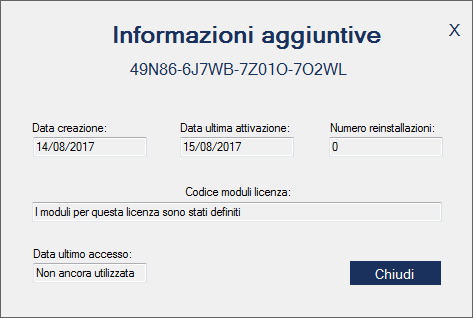
\includegraphics[width=0.7\columnwidth]{LicenseManager/ultInfo} 
    \caption{License Manager 1.0 - Creazione del codice moduli}
\label{info}
\end{figure}

Le informazioni fornite sono:

\begin{itemize}
\item \textbf{Data creazione:} data di creazione della licenza;
\item \textbf{Data ultima attivazione:} data in cui la licenza è stata attivata l’ultima volta, poiché un utente finale può disattivare e attivare una propria licenza senza limiti;
\item \textbf{Numero reinstallazioni:} quante reinstallazioni sono state eseguite dall’utente;
\item \textbf{Codice moduli licenza:} codice riepilogativo dei moduli selezionati se chi visualizza è un \textit{Admin}, altrimenti è mostrato se i moduli sono stati definiti o meno; 
\item \textbf{Data ultimo accesso:} data ultima in cui l’utente ha usato il \textit{Software Gestionale Vision} legato a quella licenza.

\end{itemize}

\subsection{Aggiorna Lista}
La funzione "Aggiorna lista" permette di ricaricare la lista delle licenze. Nel riaggiornare, è chiesto se si vogliono mantenere i filtri di ricerca eventualmente impostati in precedenza.

\subsection{Applica Filtro}
La funzione "Applica filtro" permette di applicare dei filtri sui campi delle licenze. Tra i filtri disponibili agli \textit{Admin} è selezionabile "Codice Utente", che permette di quindi di restringere il campo delle licenze visibili a quelle di un solo utente, per monitorare le licenze di un rivenditore.\\
Un filtro, in generale, è formato da tre parametri: il campo da filtrare (ad esempio \texttt{Product Key} o \texttt{Serial Number}), la condizione da applicare (ad esempio "Uguale" o "Contiene") e il valore con cui applicare il filtro.

\subsection{Rimuovi Filtro}
La funzione "Rimuovi filtro" rimuove il filtro selezionato in precedenza, tornando a mostrare tutte le licenze visibili all’utente.


%**************************************************************

\section{Esporta ed Invia}

Nella sezione "Esporta ed Invia" è possibile esportare alcuni dati relativi alle licenze o creare un documento riepilogativo della licenza selezionata. Come per la sezione "Gestione Licenze" saranno mostrate solo le licenze compatibili con il Codice Utente dell’utente loggato. I campi qui mostrati riguardano i contatti delle licenze.
In Figura \ref{espinv} è possibile vedere una situazione esempio della sezione.

\begin{figure}[!h] 
    \centering 
    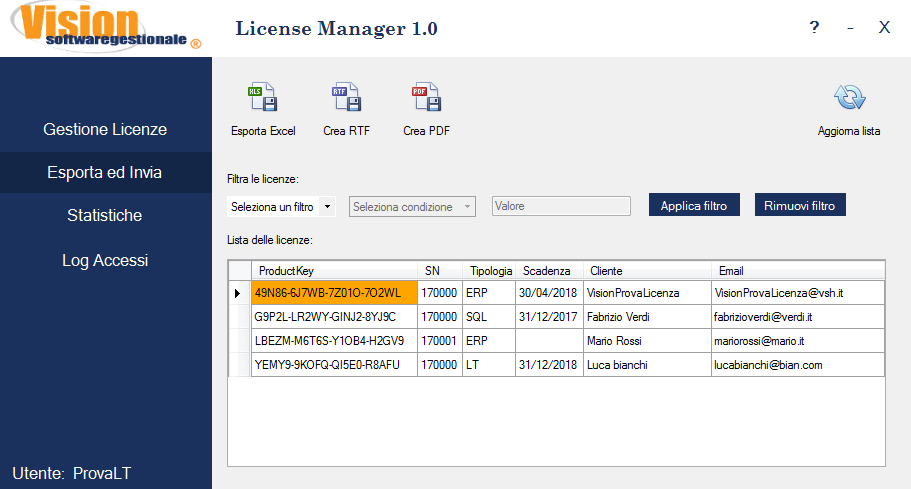
\includegraphics[width=0.9\columnwidth]{LicenseManager/esportainvia} 
    \caption{License Manager 1.0 - Sezione Esporta ed Invia}
\label{espinv}
\end{figure}

Nei paragrafi successivi sono mostrate nel dettaglio tutte le funzionalità. 

\subsection{Esporta Excel}

La funzione "Esporta Excel" permette di esportare in un file ".xls" due tipologie di dati:
\begin{itemize}

\item \textbf{Tutti i dati:} esporta tutte le licenze visibili all’utente con tutti i loro dati. Nel caso a esportare i dati fosse un \textit{Guest} non sarebbe mostrato il \texttt{Codice Moduli} e il \texttt{Codice Utente} per motivi di sicurezza.
\item \textbf{Contatti:} esporta solo i contatti riguardanti le licenze, ovvero tutti i campi visibili in questa schermata.

\end{itemize}

L'ottenimento dei dati avviene tramite l'utilizzo del Web Service \texttt{LicenseManagerService}.

\subsection{Crea RTF}
\label{creartf}
La funzione "Crea RTF" permette di creare un file RTF contenente il riepilogo della licenza da inviare al cliente al momento dell’acquisto. La creazione del file avviene secondo un file modello posto nella cartella di installazione di \textit{License Manager 1.0}. Se questo modello non è presente viene utilizzato un modello standard.

Il file modello è simile a quello mostrato in Figura \ref{modello}.

\begin{figure}[!h] 
    \centering 
    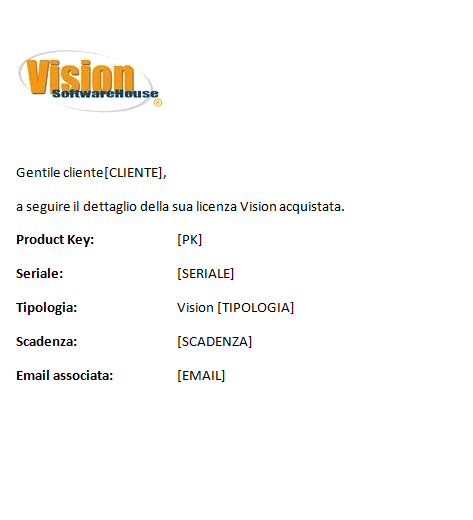
\includegraphics[width=0.7\columnwidth]{LicenseManager/modello} 
    \caption{Modello riepilogativo di una licenza}
\label{modello}

\end{figure}

Il programma sostituisce i parametri contenuti tra parentesi quadre e genera il file finale. Qualora si voglia utilizzare un nuovo modello, è sufficiente collocare le scritte tra parentesi quadre nella posizione desiderata all’interno del file e il programma provvederà a sostituirle con i valori opportuni.

\subsection{Crea PDF}

La funzione "Crea PDF" permette di creare un file PDF partendo dal modello RTF disponibile, o in caso di assenza secondo un modello standard, come spiegato nella sezione \ref{creartf}.

\subsection{Aggiorna Lista}
La funzione "Aggiorna lista" permette di ricaricare la lista delle licenze. Nel riaggiornare, è chiesto se si vogliono mantenere i filtri di ricerca eventualmente impostati in precedenza.

\subsection{Applica Filtro}
La funzione "Applica filtro" permette di applicare dei filtri sui campi delle licenze. Tra i filtri disponibili agli \textit{Admin} è selezionabile "Codice Utente", che permette di quindi di restringere il campo delle licenze visibili a quelle di un solo utente, per monitorare le licenze di un rivenditore.

\subsection{Rimuovi Filtro}
La funzione "Rimuovi filtro" rimuove il filtro selezionato in precedenza, tornando a mostrare tutte le licenze visibili all’utente.


%**************************************************************
\section{Statistiche}

Nella sezione "Statistiche" è possibile avere un quadro riassuntivo delle proprie licenze, o nel caso di un \textit{Admin} di tutte le licenze o di quelle del rivenditore selezionato.\\
In Figura \ref{stat} è possibile vedere una situazione esempio della sezione.


\begin{figure}[!h] 
    \centering 
    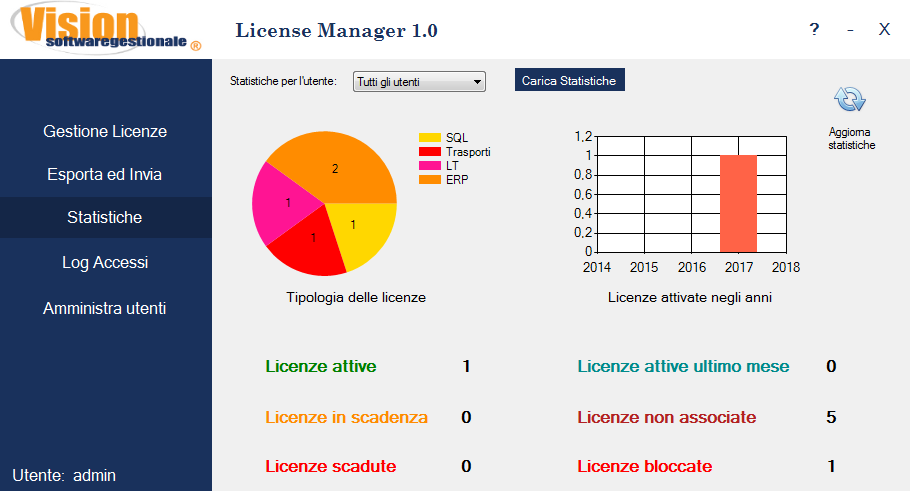
\includegraphics[width=0.9\columnwidth]{LicenseManager/statistiche} 
    \caption{License Manager 1.0 - Sezione Statistiche}
\label{stat}

\end{figure}

Attraverso la combobox "Statistiche per l’utente" (visibile ai soli \textit{Admin}) si può scegliere per quale rivenditore visualizzare le statistiche. Selezionando "Tutti gli utenti" si avranno le statistiche su tutte le licenze. È necessario cliccare su "Carica Statistiche" per applicare il filtro dell’Utente.\\
Le statistiche mostrate sono le seguenti:

\begin{itemize}

\item \textbf{Tipologia delle licenze:} grafico a torta che mostra il numero di licenze per tipologia;
\item \textbf{Licenze attivate negli anni:} grafico a barre che mostra il numero di licenze attivate per ognuno degli ultimi tre anni;
\item \textbf{Licenze attive:} quante licenze sono state attivate;
\item \textbf{Licenze in scadenza:} quante licenze scadranno nei prossimi tre mesi;
\item \textbf{Licenze scadute:} quante licenze sono scadute;
\item \textbf{Licenze attive ultimo mese:} quante licenze sono state usate nell’ultimo mese attraverso il \textit{Software Gestionale Vision};
\item \textbf{Licenze non associate:} quante licenze non hanno una componente Hardware associata;
\item \textbf{Licenze bloccate:} quante licenze sono bloccate.

\end{itemize}

L'ottenimento delle statistiche avviene tramite l'utilizzo del Web Service \textit{LicenseManagerService}.

%**************************************************************
\section{Log Accessi}

Nella sezione "Log Accessi" è possibile monitorare gli accessi al \textit{Software Gestionale Vision}, legando al \texttt{Product Key} utilizzato per l’attivazione l’indirizzo IP e il MAC Address della scheda di rete utilizzati per connettersi a Internet. In questo modo è possibile venire a conoscenze di alcune anomalie come accessi multipli da diverse postazioni, qualora i controlli fossero stati evasi.\\
In Figura \ref{accessi} è possibile vedere una situazione esempio della sezione.
\begin{figure}[!h] 
    \centering 
    \includegraphics[width=0.9\columnwidth]{LicenseManager/logAccessi} 
    \caption{License Manager 1.0 - Sezione Log Accessi}
\label{accessi}

\end{figure}

\subsection{Funzionalità}

Sotto le voci "Licenze con multipli IP" e "Licenze con multipli MAC Address" sono mostrate quante licenze hanno rispettivamente più indirizzi IP e più MAC Address associati.
Se una licenza dovesse avere più di due indirizzi associati verrebbe contata comunque una sola volta.\\
Cliccando su "Licenze con multipli IP" vengono selezionati in verde il \texttt{Product Key} e \texttt{l’indirizzo IP} dei record che hanno un \texttt{indirizzo IP} diverso dalla prima occorrenza per quel \texttt{Product Key}.\\
Cliccando su "Licenze con multipli MAC Address" vegono selezionati in rosso il \texttt{Product Key} e il \texttt{MAC Address} dei record che hanno un \texttt{MAC Address} diverso dalla prima occorrenza per quel \texttt{Product Key}.
In caso una licenza avesse sia diverso \texttt{indirizzo IP} sia diverso \texttt{MAC Address} il \texttt{Product Key} è evidenziato in viola.\\
Il funzionamento illustrato in precedenza è mostrato nella Figura \ref{multip}.

\begin{figure}[!h] 
    \centering 
    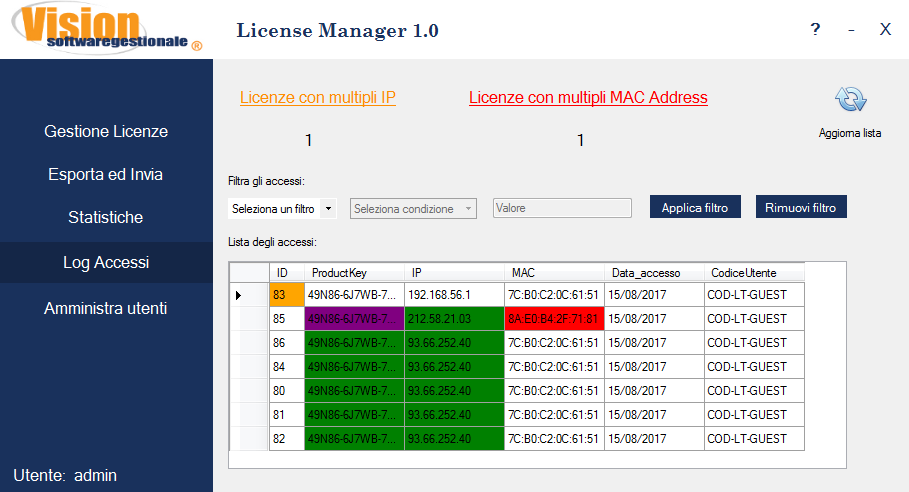
\includegraphics[width=0.9\columnwidth]{LicenseManager/multip} 
    \caption{License Manager 1.0 - Selezione delle licenze con multipli IP e MAC Address}
\label{multip}

\end{figure}

Gli accessi al \textit{Software Gestionale Vision} sono ottenuti tramite l'utilizzo del Web Service \texttt{LicenseManagerService}.


%**************************************************************
\section{Amministra Utenti}

La sezione "Amministra utenti" è visibile ai soli utenti \textit{Admin} e permette di gestire gli utenti del programma \textit{License Manager 1.0}.\\
In Figura \ref{amm} è possibile vedere una situazione esempio della sezione.
\begin{figure}[!h] 
    \centering 
    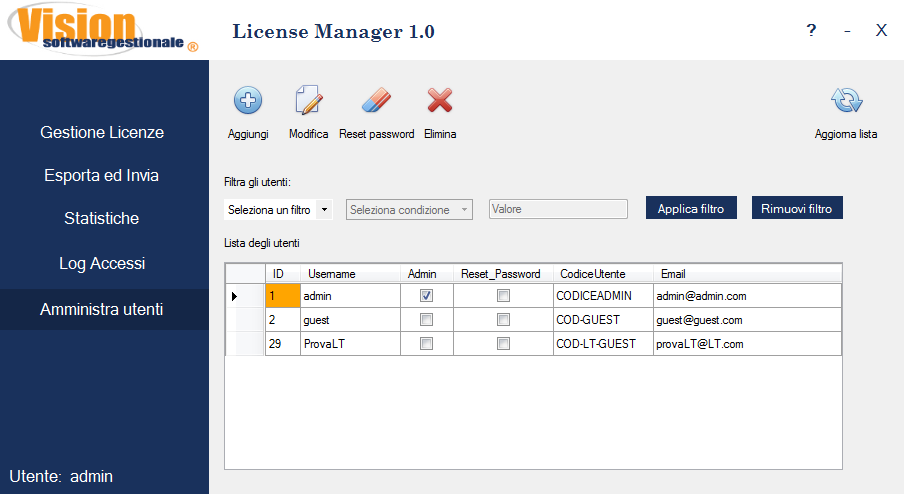
\includegraphics[width=0.9\columnwidth]{LicenseManager/amministra} 
    \caption{License Manager 1.0 - Sezione Amministra Utenti}
\label{amm}

\end{figure}

Nella parte alta della schermata sono presenti le funzionalità, mentre nella parte bassa è mostrata la lista degli utenti con le loro caratteristiche.\\
Nello specifico le operazioni permesse, nell'ordine, sono:
\begin{itemize}
\item \textbf{Aggiungi:} permette di creare un nuovo utente;
\item \textbf{Modifica:} permette di modificare un utente;
\item \textbf{Reset password:} concede o rimuove la possibilità di un utente di resettare la propria password;
\item \textbf{Elimina:} permette di eliminare un utente.
\end{itemize}

Nei paragrafi successivi sono mostrate nel dettaglio tutte le funzionalità. 

\subsection{Aggiungi}


La funzione "Aggiungi" permette di creare un nuovo utente. La finestra che si presenta è mostrata in Figura \ref{agg}.

\begin{figure}[!h] 
    \centering 
    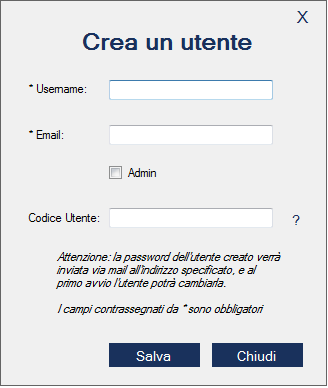
\includegraphics[width=0.4\columnwidth]{LicenseManager/aggut} 
    \caption{License Manager 1.0 - Creazione di un utente}
\label{agg}

\end{figure}

I campi Username ed Email sono obbligatori.
\begin{itemize}
\item \textbf{Username:} identifica univocamente un utente, credenziale necessaria per l’accesso;
\item \textbf{Email:} lega un utente a una mail, che sarà utilizzata sia per l’invio della password da utilizzare per il primo accesso sia per le notifiche di creazione di nuove licenze da parte di un rivenditore.
\end{itemize}
Il campo \texttt{Admin}, se selezionato, identifica l’utente come \textit{Admin}, fornendone tutti i privilegi.\\
Il \texttt{Codice Utente} è deciso manualmente alla creazione o in seguito attraverso la funzione di modifica utente, e serve per identificare un utente con il proprio codice rivenditore. Più utenti possono avere lo stesso \texttt{Codice Utente}, e saranno quindi in grado di gestire le stesse licenze. Gli \textit{Admin} hanno il \texttt{Codice Utente} sempre impostato a "CODICEADMIN", il che gli differenzia dagli altri utenti \textit{Guest}.\\
Dopo aver salvato l’utente, tramite l'utilizzo del Web Service \texttt{LicenseManagerService} è inviata una Mail all’indirizzo scelto contenente l’username e la password da utilizzare per il primo accesso. Dopo l’accesso, è richiesto l’inserimento di una nuova password per questioni di sicurezza.


\subsection{Modifica}

La funzione "Modifica" permette di modificare un utente. La finestra che si presenta è mostrata in Figura \ref{mod}.

\begin{figure}[!h] 
    \centering 
    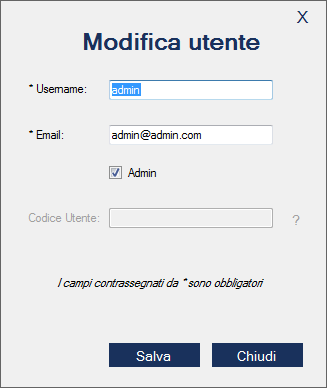
\includegraphics[width=0.4\columnwidth]{LicenseManager/modut} 
    \caption{License Manager 1.0 - Modifica di un utente}
\label{mod}

\end{figure}

Con questo Form può essere modificato l’username, l'indirizzo email associato all’account e fornire o rimuovere i privilegi di \textit{Admin}. Qualora l’utente sia un \textit{Admin} non è possibile scegliere un \texttt{Codice Utente} poiché sarà impostato di default a "CODICEADMIN".

\subsection{Reset password}

La funzione "Reset password" permette all’utente selezionato di poter reimpostare la password alla prossima autenticazione. Il reset della password deve avvenire sempre tramite il permesso di un \textit{Admin}, e non sono previsti altri metodi.
\\
Per resettare la password qualora l’utente non ricordasse la vecchia, è sufficiente inserire l’\texttt{Username} nel campo apposito del Form di autenticazione e cliccare su "Password dimenticata?".\\
È possibile per un Admin resettare la propria password seguendo la stessa procedura, scegliendone una nuova al prossimo accesso.
\\
In Figura \ref{reset} è mostrato il processo di reset della password tramite il Form di autenticazione.

\begin{figure}[!h] 
    \centering 
    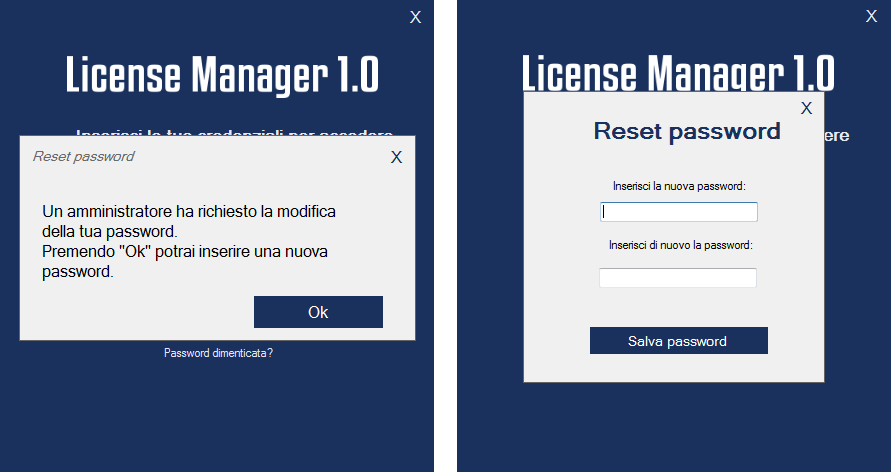
\includegraphics[width=1\columnwidth]{LicenseManager/reset} 
    \caption{License Manager 1.0 - Reset della password di un utente}
\label{reset}

\end{figure}


\newpage
\subsection{Elimina}

La funzione "Elimina" permette di eliminare un utente di \textit{License Manager 1.0}, tranne se stessi. Per eliminare un \textit{Admin} è necessario svolgere l’operazione da un altro account \textit{Admin}. Poiché l’eliminazione è sempre permessa, si consiglia di limitare al minimo il numero di utenti \textit{Admin} presenti.             % Product Prototype
% !TEX encoding = UTF-8
% !TEX TS-program = pdflatex
% !TEX root = ../tesi.tex

%**************************************************************
\chapter{Moduli Software Gestionale Vision}
\label{cap:moduli-vision}
%**************************************************************



%**************************************************************
\section{Premesse}


%**************************************************************
\section{Registrazione della licenza}


%**************************************************************
\section{Avvio del software in modalità Online}


%**************************************************************
\section{Avvio del software in modalità Offline}


%**************************************************************
\section{Controllo della licenza durante l'esecuzione}


%**************************************************************
\section{Disattivazione della licenza}


%**************************************************************
\section{Modifica dell'indirizzo email della licenza}             % Product Design Freeze e SOP
% !TEX encoding = UTF-8
% !TEX TS-program = pdflatex
% !TEX root = ../tesi.tex

%**************************************************************
\chapter{Analisi retrospettiva}
\label{cap:analisi-retrospettiva}
%**************************************************************
Questo capitolo analizza l'attività di stage rispetto agli obiettivi raggiunti, ai benefici che le soluzioni ideate porteranno all'azienda e alle considerazioni finali dell'attività svolta.


%**************************************************************
\section{Obiettivi Raggiunti}

Gli obiettivi primari prefissati nel piano di lavoro sono stati completamente raggiunti. In seguito ad un'accurata analisi delle problematiche da risolvere è stato redatto un documento informale contenente a grandi linee le soluzioni che si intendevano sviluppare. Una volta approvate dal tutor aziendale, esse sono state sviluppate utilizzando dei Web Service come richiesto. Attraverso i moduli da aggiungere al \textit{Software Gestionale Vision} sono ora presenti dei nuovi metodi di attivazione e disattivazione delle licenze, seguiti dai controlli di validità. La creazione è invece gestita da \textit{License Manager 1.0}, rimpiazzando il Software \textit{GenPK} ed eliminando le problematiche ad esso correlate.
\\Anche gli obiettivi secondari e facoltativi sono stati raggiunti con successo. La data di scadenza può essere gestita da \textit{License Manager 1.0} e nella fase di avvio del \textit{Software Gestionale Vision} essa è controllata. Sempre tramite \textit{License Manager 1.0} è possibile gestire i moduli di una licenza, eliminando l'utilizzo del programma \textit{GenFileKey} e dei problemi ad esso correlati. Tramite la sezione "Log Accessi" del programma è possibile avere una panoramica completa dell'utilizzo diel \textit{Software Gestionale Vision} comprese le anomalie, e nella sezione "Statistiche" è possibile osservare i dati riguardanti le licenze utili per scopi gestionali e di marketing.
\\Oltre agli obiettivi presentati nel piano di lavoro, durante lo stage ne sono stati fissati degli altri, grazie ad un veloce apprendimento delle tecnologie e a una buona progettazione. Attraverso \textit{License Manager 1.0} è stato deciso di poter gestire tutte le caratteristiche di una licenza, come un eventuale blocco, le componenti Hardware e l'indirizzo Email associato. Infine, poichè il programma è stato sviluppato utilizzando un sistema di utenti e presentava funzionalità spesso richieste anche dai rivenditori dell'azienda è stato deciso di modificare alcune sezioni per poter distribuire il Software ai rivenditori.
\\Il raggiungimento degli obiettivi formativi è illustrato nelle conclusioni.

%**************************************************************
\section{Benefici dello stage per l'azienda}
L'azienda, tramite l'attività di stage, può ora usufruire di un nuovo sistema di gestione e controllo delle proprie licenze, avendo i seguenti benefici:
\begin{itemize}
\item i problemi riguardanti le modalità di creazione delle licenze (inclusi i loro moduli) sono stati risolti;
\item è ora molto più difficile eludere la sicurezza come utilizzare licenze bloccate o la stessa licenza su più macchine grazie ai tre diversi controlli implementati (Online, Offline e durante l'esecuzione);
\item l'azienda, tramite \textit{License Manager 1.0} può ora gestire efficacemente con un solo Software le proprie licenze. Può infatti creare una licenza, gestirne i moduli, bloccarla, eliminarla, disattivarla e gestirne qualsiasi caratteristica tramite un'interfaccia semplice e intuitiva. Ha anche a disposizione un nuovo sistema di monitoraggio che permette di controllare possibili anomalie e avere informazioni utili per migliorare i propri prodotti;
\item i clienti possono gestire con maggiore autonomia la propria licenza, disattivandola e attivandola senza dover contattare l'azienda, anche in situazioni complicate come la rottura del proprio PC;
\item i rivenditori, attraverso \textit{License Manager 1.0}, possono gestire le licenze da loro vendute senza dover richiedere costantemente l'intervento di \textit{VISIONEIMPRESA s.r.l}. Le operazioni permesse ai rivenditori sono comunque ideate per preservare la sicurezza dell'azienda e ogni operazione è registrata e notificata all'azienda tramite email.
\end{itemize}

È infine importante sottolinere che avendo utlizzato dei Web Service e un Database per sviluppare le soluzioni previste è relativamente facile apportare modifiche all'intero sistema.

%**************************************************************
\section{Conclusioni}

L'esperienza di stage svolta è stata per me molto positiva. Entrare a contatto con programmatori esperti e con il mondo del lavoro è un esperienza sicuramente molto formativa che non può essere insegnata in un contesto universitario. Anche la fase di progettazione e discussione con il tutor aziendale sulle soluzioni da me proposte sono state stimolanti, poiché analizzare i benefici e gli svantaggi di una decisione aiutano a migliorare le proprie capacità progettuali.
\\Il poter creare da zero un sistema di gestione e controllo mi ha aiutato a migliorare le mie capacità decisionali e di apprendimento, soprattutto perchè nessun vincolo stretto era stato imposto. La creazione infatti, secondo me, è molto più stimolante della modifica, e per questo ho affrontato lo stage soddisfatto di quello che stavo creando, chiedendo aiuto ai programmatori più esperti in caso di difficoltà importanti e confrontandomi con il tutor aziendale per valutare la bontà delle soluzioni da me proposte.
\\A livello tecnologico ho acquisito una buona padronanza del linguaggio C\# e degli altri strumenti utilizzati nel corso dell'attività. Inoltre, entrando a contatto con un Software gestionale di buona qualità ho potuto acquisire conoscenze che mi saranno utili qualora volessi specializzarmi in questo settore.
\\L'unica nota negativa è da riferirsi alla posizione per me scomoda dell'azienda (circa quaranta minuti di auto da Padova centro), ma, poichè ho trovato il progetto molto interessante e grazie anche agli apprezzamenti ricevuti dal tutor aziendale alla fine dei lavori, sono particolarmente soddisfatto dell'attività di stage svolta.             % Conclusioni
\appendix                               
% !TEX encoding = UTF-8
% !TEX TS-program = pdflatex
% !TEX root = ../tesi.tex

%**************************************************************
\chapter{Appendice A - Grado di compatibilità}
\label{cap:appA}
%**************************************************************

Nel caso in esame per dare la possibilità al cliente di modificare alcune componenti del suo PC senza risultare di utilizzare un computer diverso, è calcolato il grado di compatibilità delle due componenti Hardware invece di verificare che siano identiche.\\ 
L'algoritmo si basa sull'idea di assegnare dei pesi alle componenti del PC in base alla probabilità che esse vengano cambiate. Più una componente è fondamentale, più peso avrà. Alla fine dei controlli è calcolato il punteggio ottenuto come somma dei pesi delle parti cambiate. Se il punteggio supera la soglia massima il computer risulta diverso.
\\Per assicurare una buona efficienza di questo metodo sono state scelte molte componenti di un computer, anche non fondamentali. I pesi sono stati attribuiti accuratamente e pensando a possibili situazioni reali.
\\Per motivi di sicurezza le componenti scelte per il controllo non sono esposte in questo documento.




             % Appendice A

%**************************************************************
% Materiale finale
%**************************************************************
\backmatter
\printglossaries
% !TEX encoding = UTF-8
% !TEX TS-program = pdflatex
% !TEX root = ../tesi.tex

%**************************************************************
% Bibliografia
%**************************************************************

\cleardoublepage
\chapter{Bibliografia}

\nocite{*}
% Stampa i riferimenti bibliografici
\printbibliography[heading=subbibliography,title={Riferimenti bibliografici},type=book]

% Stampa i siti web consultati
\printbibliography[heading=subbibliography,title={Siti web consultati},type=online]


\end{document}